\subsection{Subjective data}

There were 3 different questionnaires in this experiment. Each of these questionnaires was meant to verify one of the experiment goals:

\begin{itemize}
    \item \nameref{subsubsec:results_nasa_tlx_1};
    
        Meant to verify the mental workload of the user. Is expected that after each “First” round, the mental workload would decrease and that one of the methods would have the least mental workload.

    \item \nameref{subsubsec:results_adapted_sagat_1};
    
        Meant to verify the situation awareness and the mental map of the user. Is expected to notice an increase from the “First” round to the “Return” round at each method.

    \item \nameref{subsubsec:results_questionnaires}.

        Meant to assess the user experience with each method.

\end{itemize}

\subsubsection{NASA-TLX}
\label{subsubsec:results_nasa_tlx_1}

The NASA-TLX provides two relevant pieces of information to the workload analysis. The first is the score attributed to the "mental demand" dimension and the second is the average obtained from NASA-TLX's six dimensions. The two analyses are presented in the next subsections.

\paragraph{Analysis of the mental demand scale}\mbox{}\\

Table \ref{tab:md_table_blind} presents the "mental demand" score of each blind participant to each guidance method. The "base" method refers to the guidance method that the person uses in his/her daily life (e.g., white cane). 


\begin{table}[!htb]
\centering
\caption{Score of NASA-TLX mental demand for the blind participants.}
\label{tab:md_table_blind}
\begin{tabular}{llrrrrr}
\toprule
     &        & Base & Audio & \begin{tabular}[c]{@{}l@{}}Haptic\\ Belt\end{tabular} & \begin{tabular}[c]{@{}l@{}}Virtual\\ Cane\end{tabular} & Mixture \\
Participant & Round &      &       &                                                       &                                                        &         \\
\midrule
001C & First &    3 &     1 &                                                    14 &                                                      3 &       6 \\
     & Return &    1 &     1 &                                                    10 &                                                      2 &       6 \\
002C & First &    5 &     1 &                                                     1 &                                                     10 &      12 \\
     & Return &    1 &     1 &                                                     1 &                                                     10 &       3 \\
003C & First &    5 &     5 &                                                     5 &                                                      8 &       1 \\
     & Return &    3 &     1 &                                                     1 &                                                      2 &       1 \\
004C & First &    9 &    10 &                                                    15 &                                                     10 &      10 \\
     & Return &    7 &    10 &                                                    14 &                                                      8 &      10 \\
\bottomrule
\end{tabular}
\end{table}



The mean value obtained for each guidance method is illustrated in Figure \ref{fig:barplot_md_avg_5_scene_blind}. It shows a systematic reduction in the perceived mental workload between the rounds for all methods, confirming that the participants get familiar with the devices after the first use. It also shows that although the haptic belt obtained the most considerable mean, it also had the most significant variation, showing that the effort required from the user may vary significantly.

\begin{figure}[!htb]
    \centering
    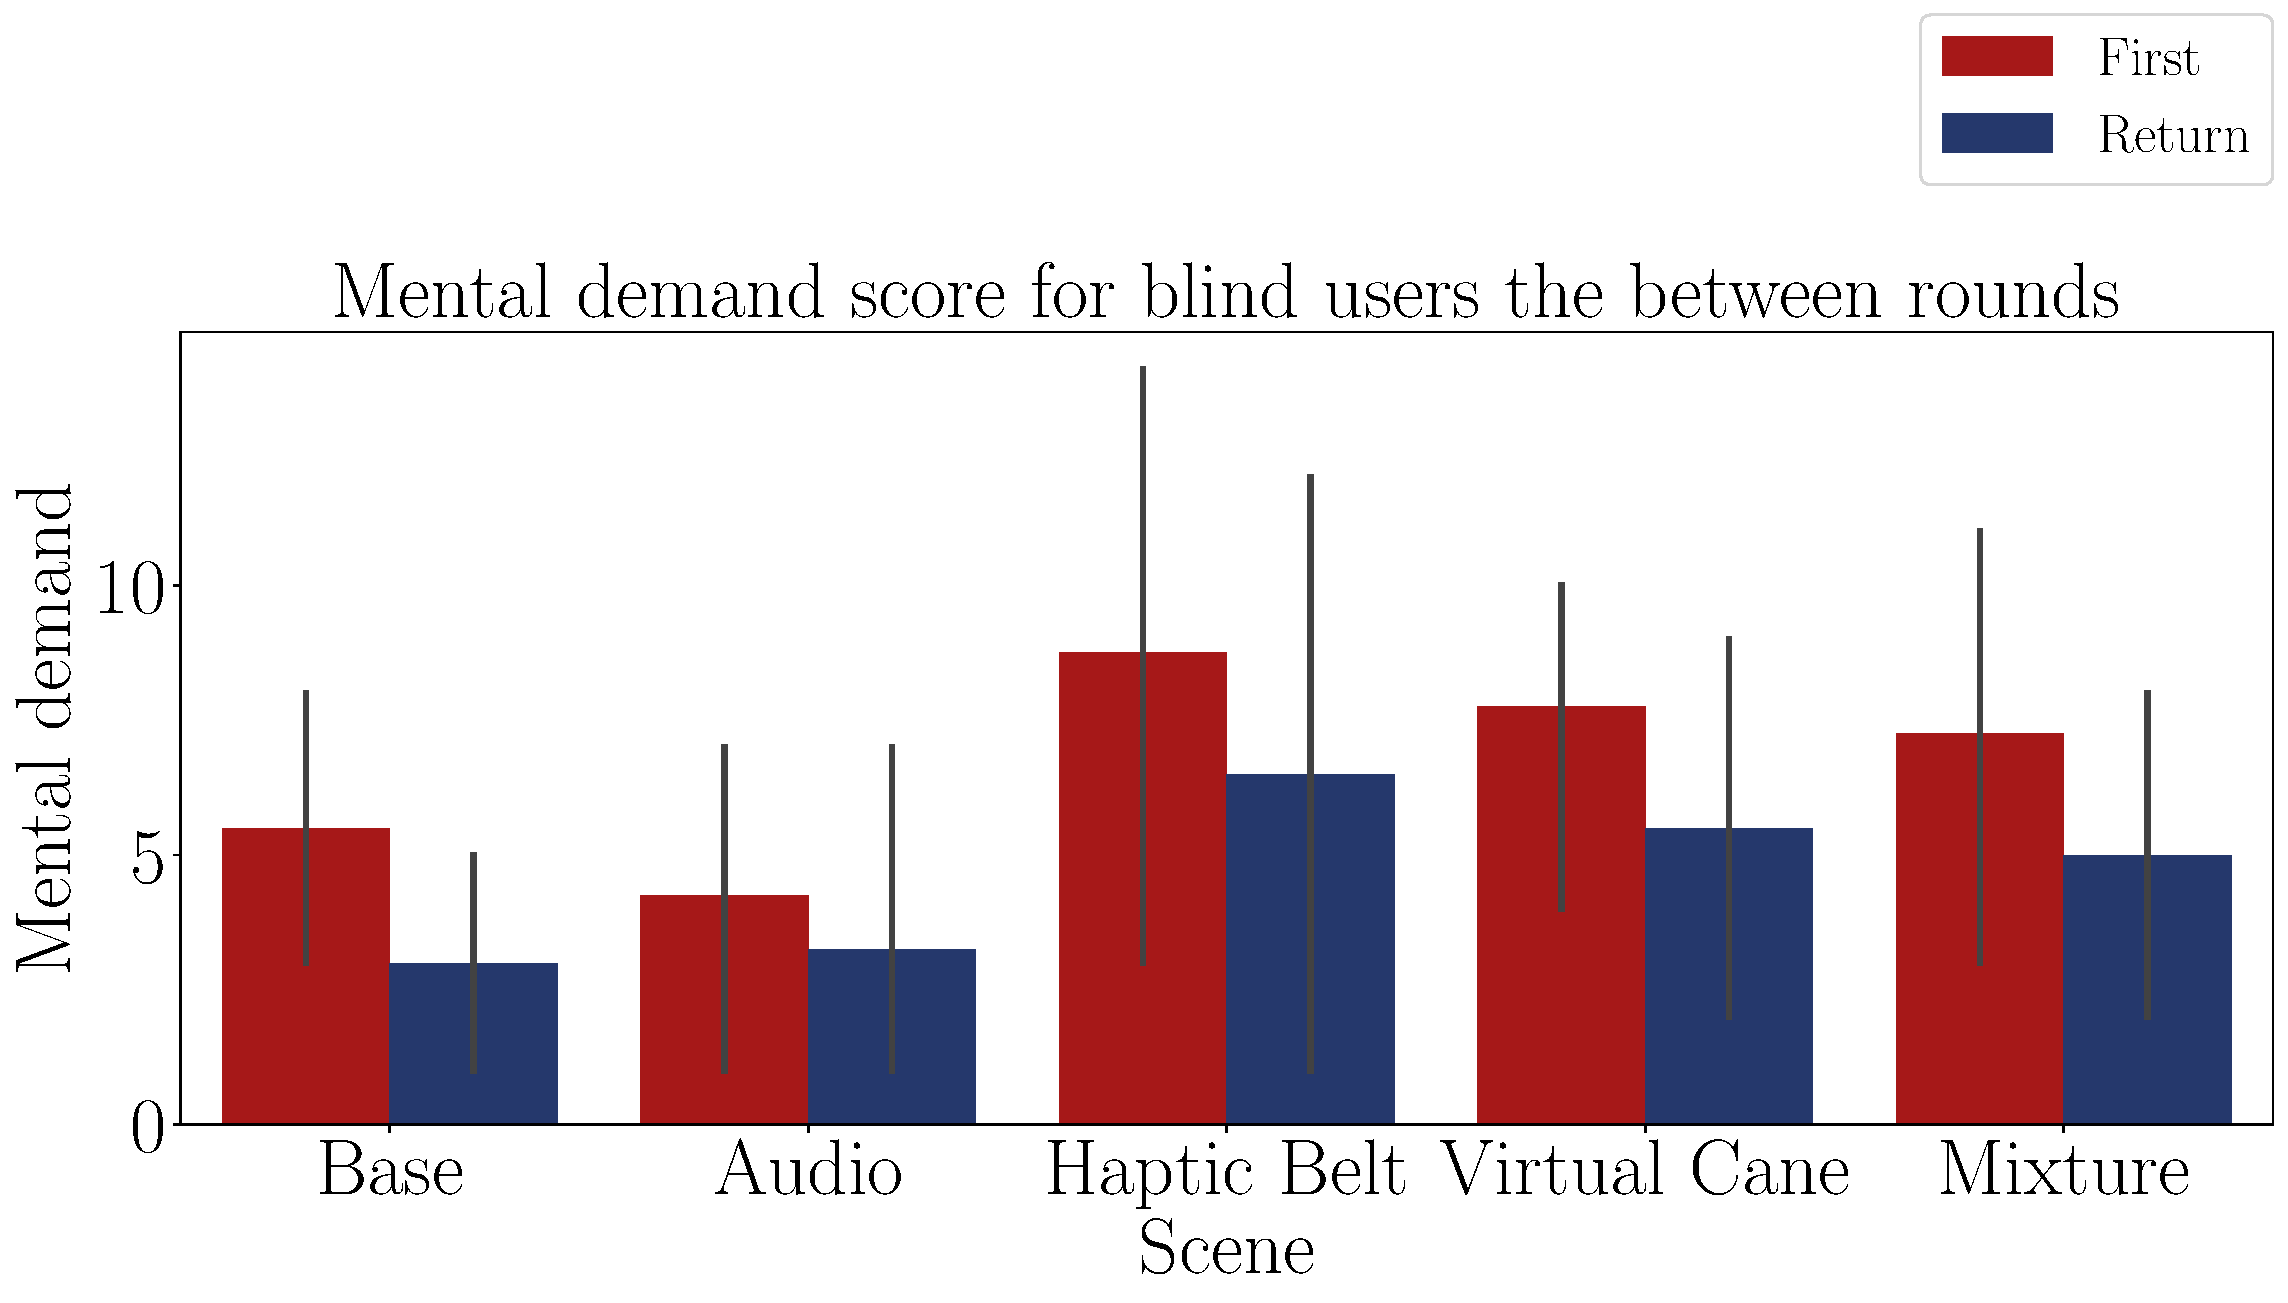
\includegraphics[width = \textwidth]{Resultados/Nasa/Figuras/pdf/barplot_md_avg_5_scene_blind.pdf}
    \caption{Mean and standard deviation of mental demand of blind participants for each method.}
    \label{fig:barplot_md_avg_5_scene_blind}
\end{figure}


Figure \ref{fig:boxplot_md_blind_scene}  presents a boxplot of the mental demand score grouped by the methods. This figure shows that there may be two groups: one associated with lower demand, composed of "base" and "audio", and another with higher demand, composed of "haptic belt", "virtual cane" and "mixture". It indicates that maybe a guidance method that uses vibration as input is not intuitive. Figure \ref{fig:boxplot_md_blind_rounds} presents a boxplot of the mental demand grouped by the rounds, confirming the general tendency to reduce the required "mental demand". 

\begin{figure}[!htb]
    \centering
    \begin{minipage}{0.45\textwidth}
        \centering
        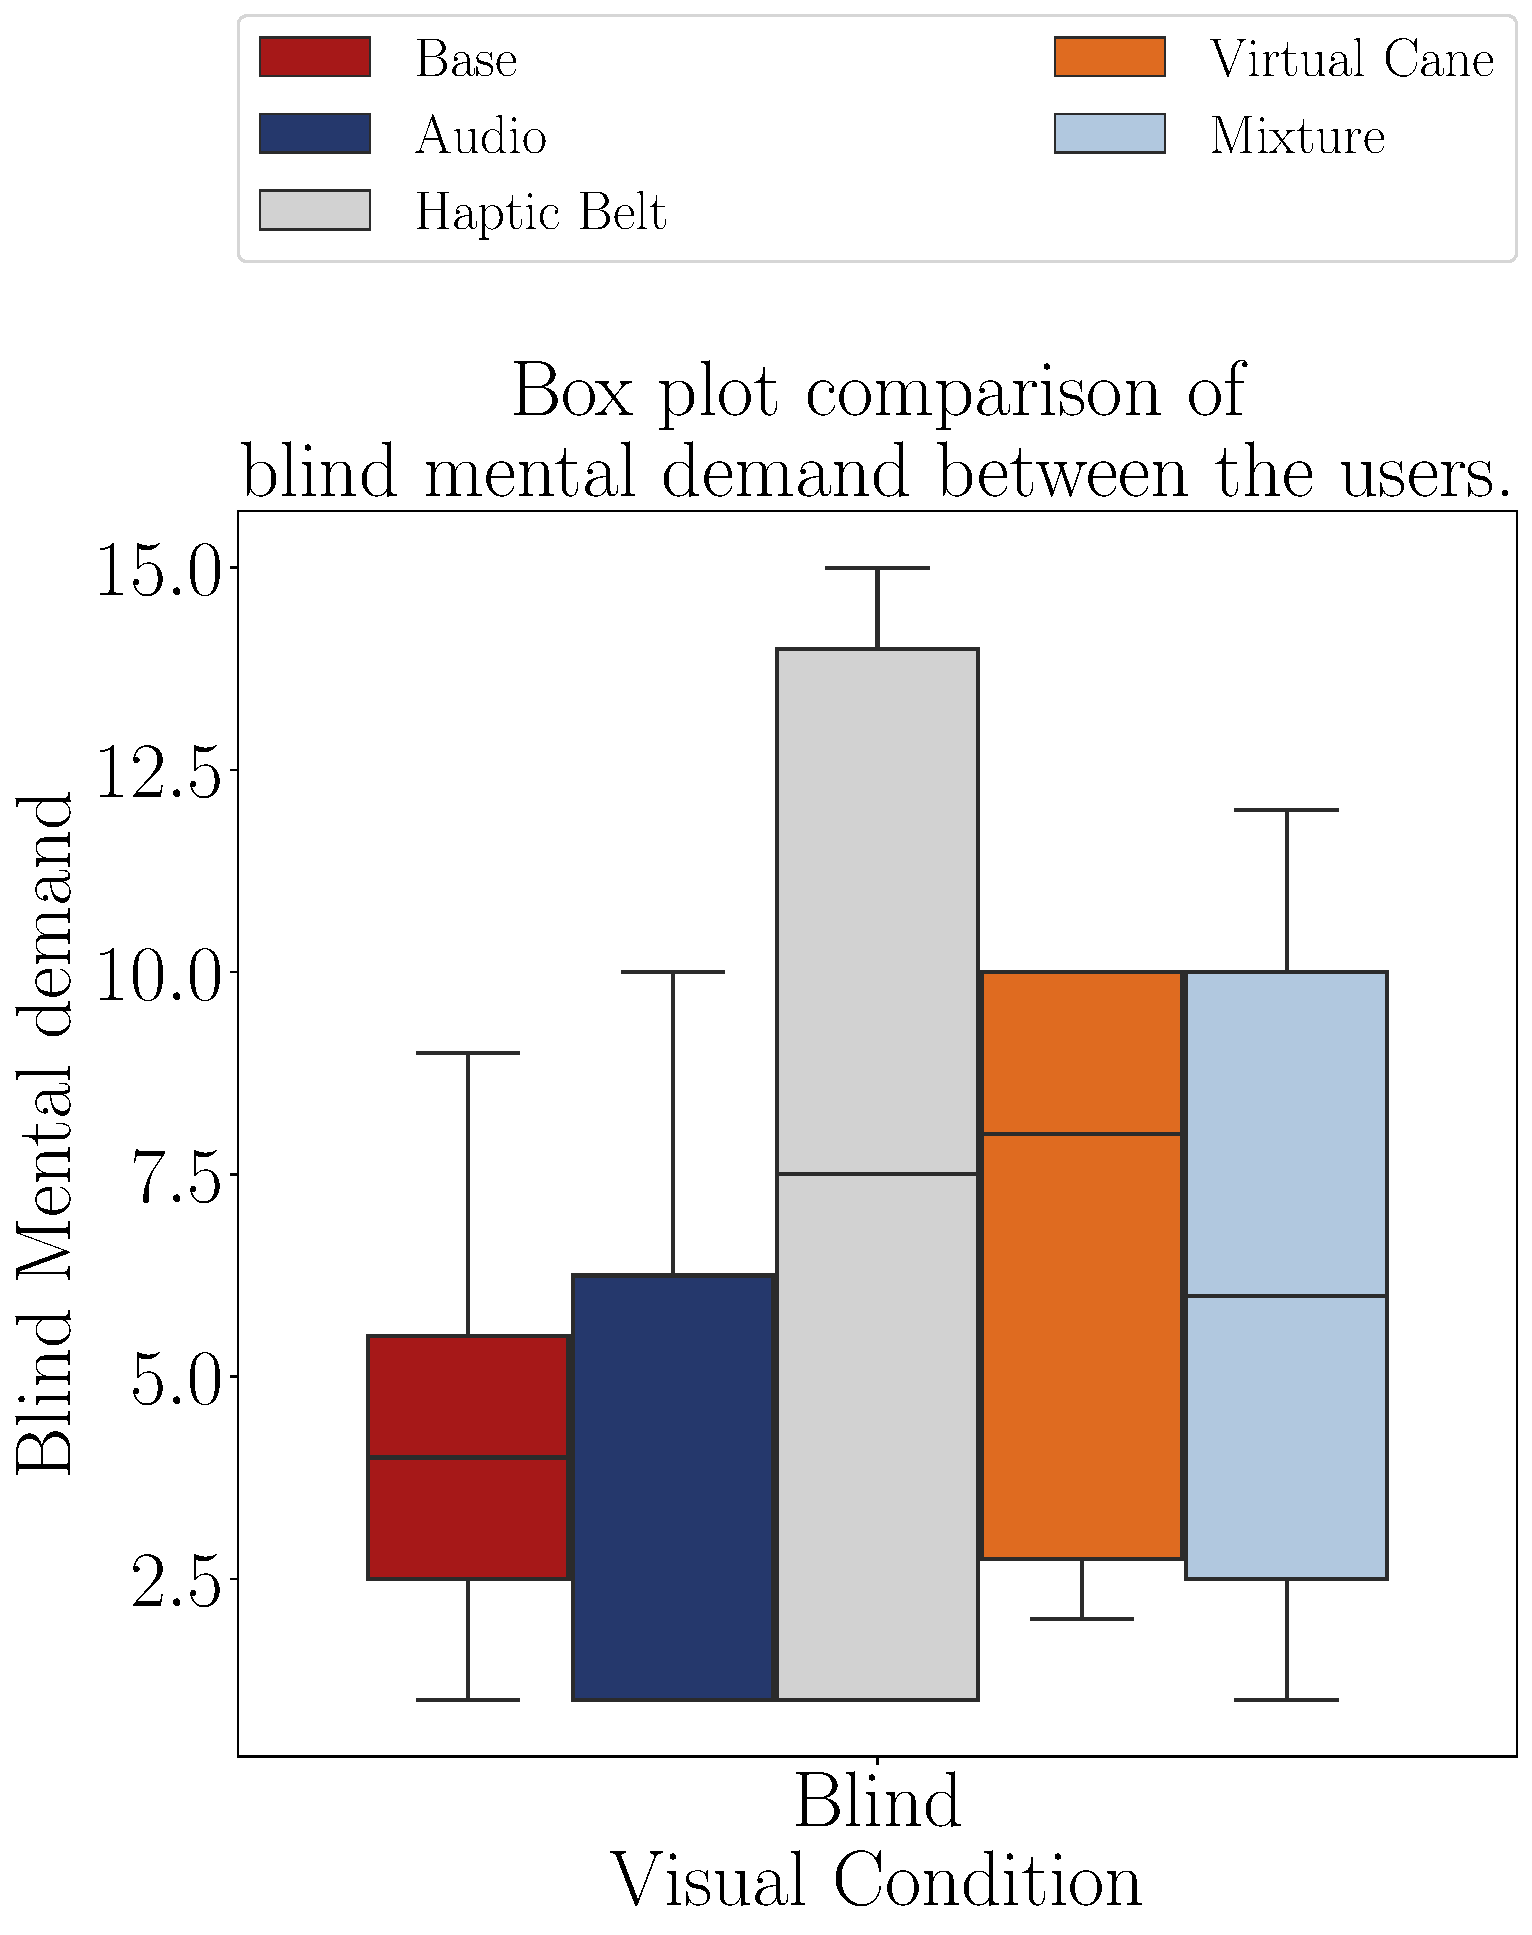
\includegraphics[width = \textwidth]{Resultados/Nasa/Figuras/pdf/boxplot_md_blind_scene.pdf}
        \caption{Boxplot of the mental demand of the blind participants grouped by the methods.}
        \label{fig:boxplot_md_blind_scene}
    \end{minipage}
    \begin{minipage}{0.075\textwidth}
        \hfill
    \end{minipage}
    \begin{minipage}{0.45\textwidth}
        \centering
        %\vspace{3ex}
        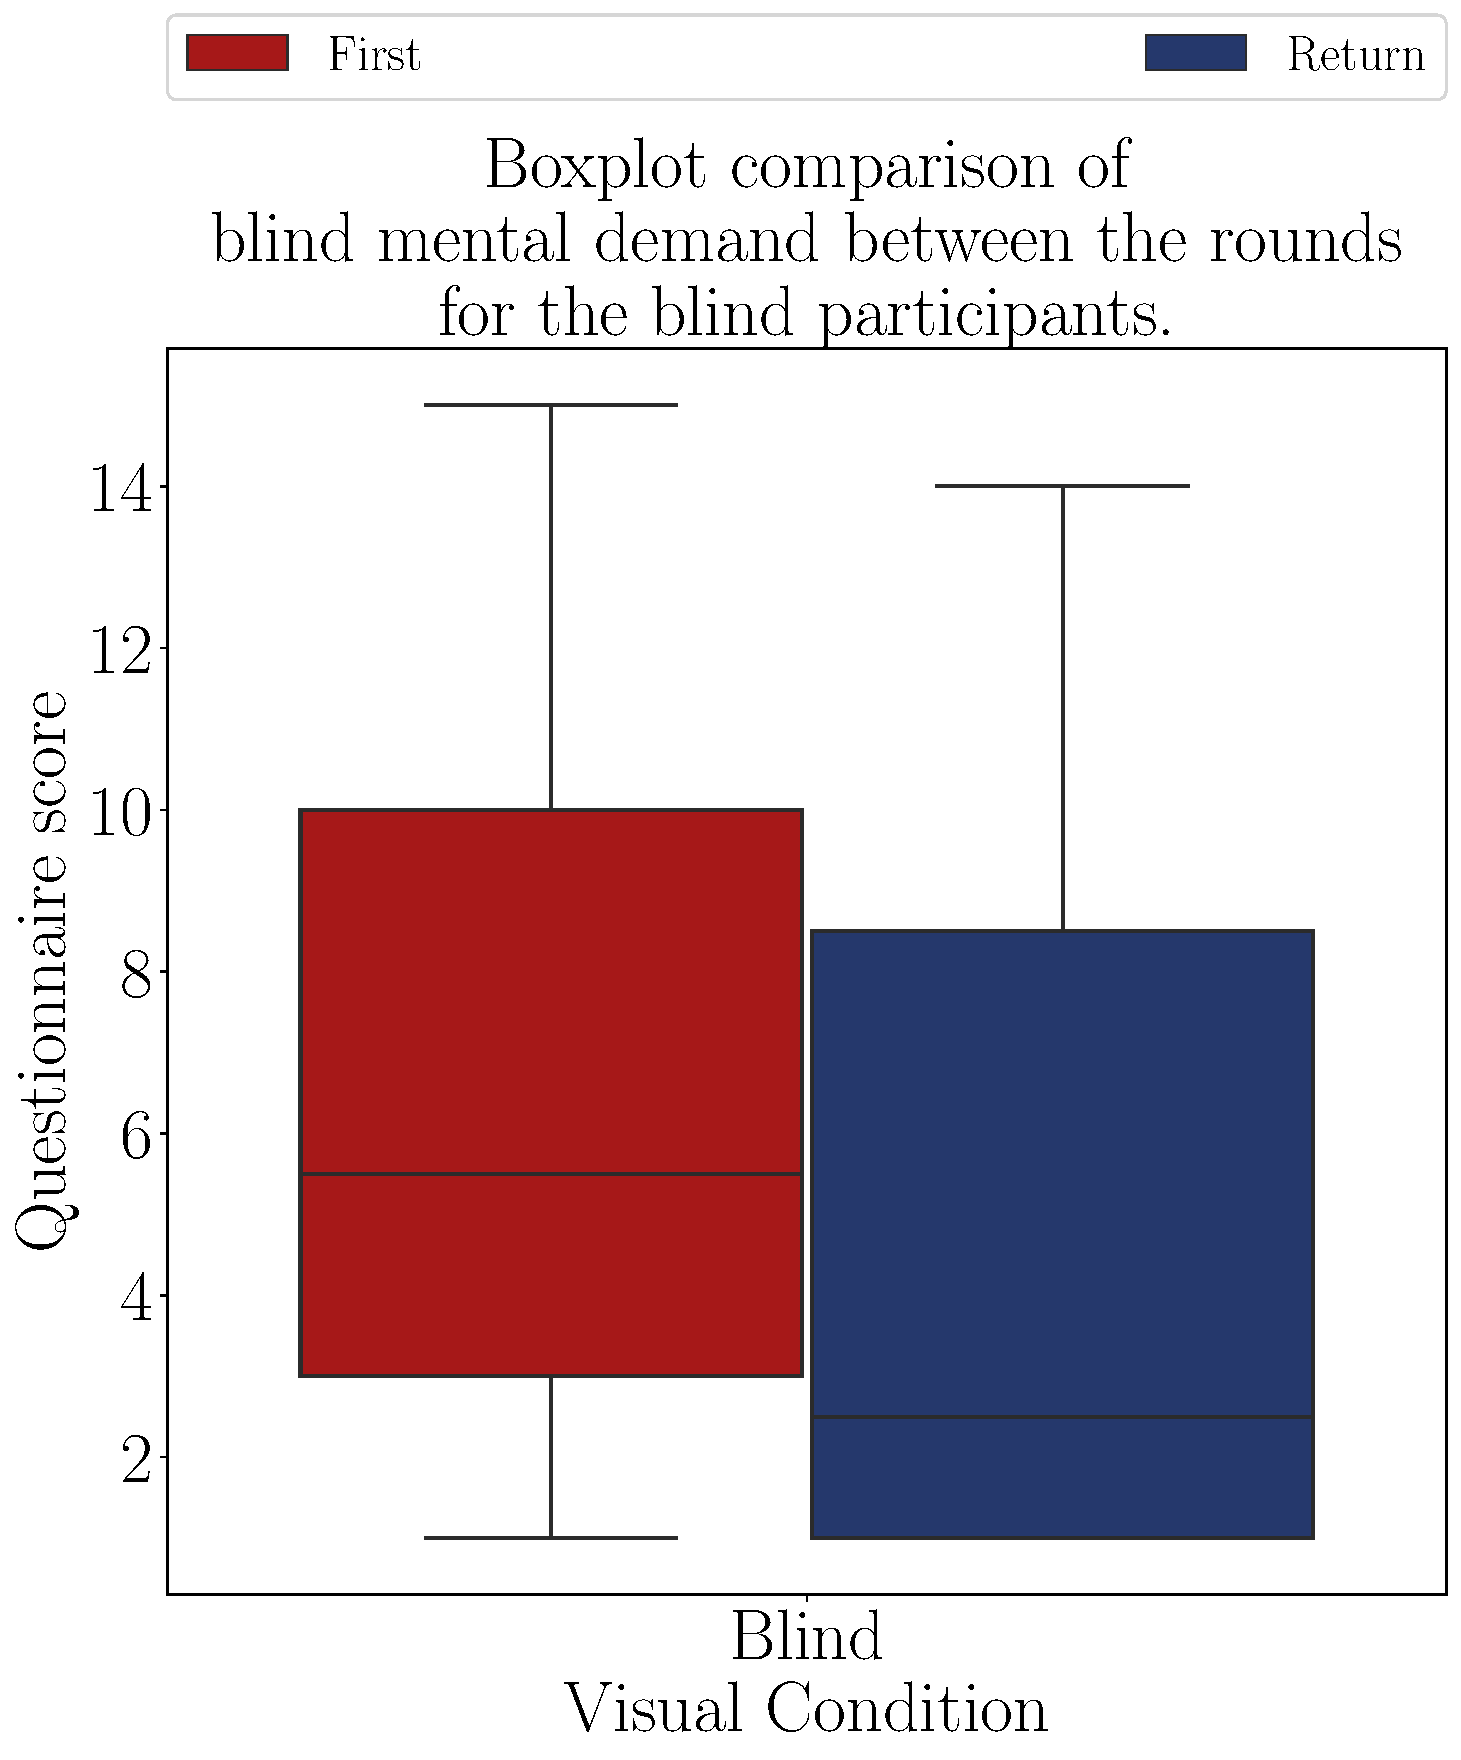
\includegraphics[width = \textwidth]{Resultados/Nasa/Figuras/pdf/boxplot_md_blind_rounds.pdf}
        \caption{Boxplot of the mental demand of the blind participants grouped by the round.}
        \label{fig:boxplot_md_blind_rounds}
    \end{minipage}
\end{figure}

In order to support the statistical analysis, Figures \ref{fig:qqplot_md_avg_two_way_blind} and \ref{fig:residplot_md_avg_two_way_blind} presents the QQ-plot and the residual plot of the "mental demand" data, confirming that the data follow a normal distribution and the residues are homogenous.

Figures \ref{fig:qqplot_md_avg_two_way_blind} and \ref{fig:residplot_md_avg_two_way_blind} show the distribution and variance of Table \ref{tab:md_table_blind}. These figures show that the data are normally distributed and that the methods have a similar variance. Table \ref{tab:blocanova_md_avg_two_way_blind} shows the ANOVA test p-values of the mental demand of the "blind” sample between the guidance methods. The methods' and the rounds' p-values indicate that there is no influence from them in the mental demand. The interaction between the methods and the round also does not influence the mental demand.

\begin{figure}[!htb]
    \centering
    \begin{minipage}{0.45\textwidth}
        \centering
        %\vspace{1ex}
        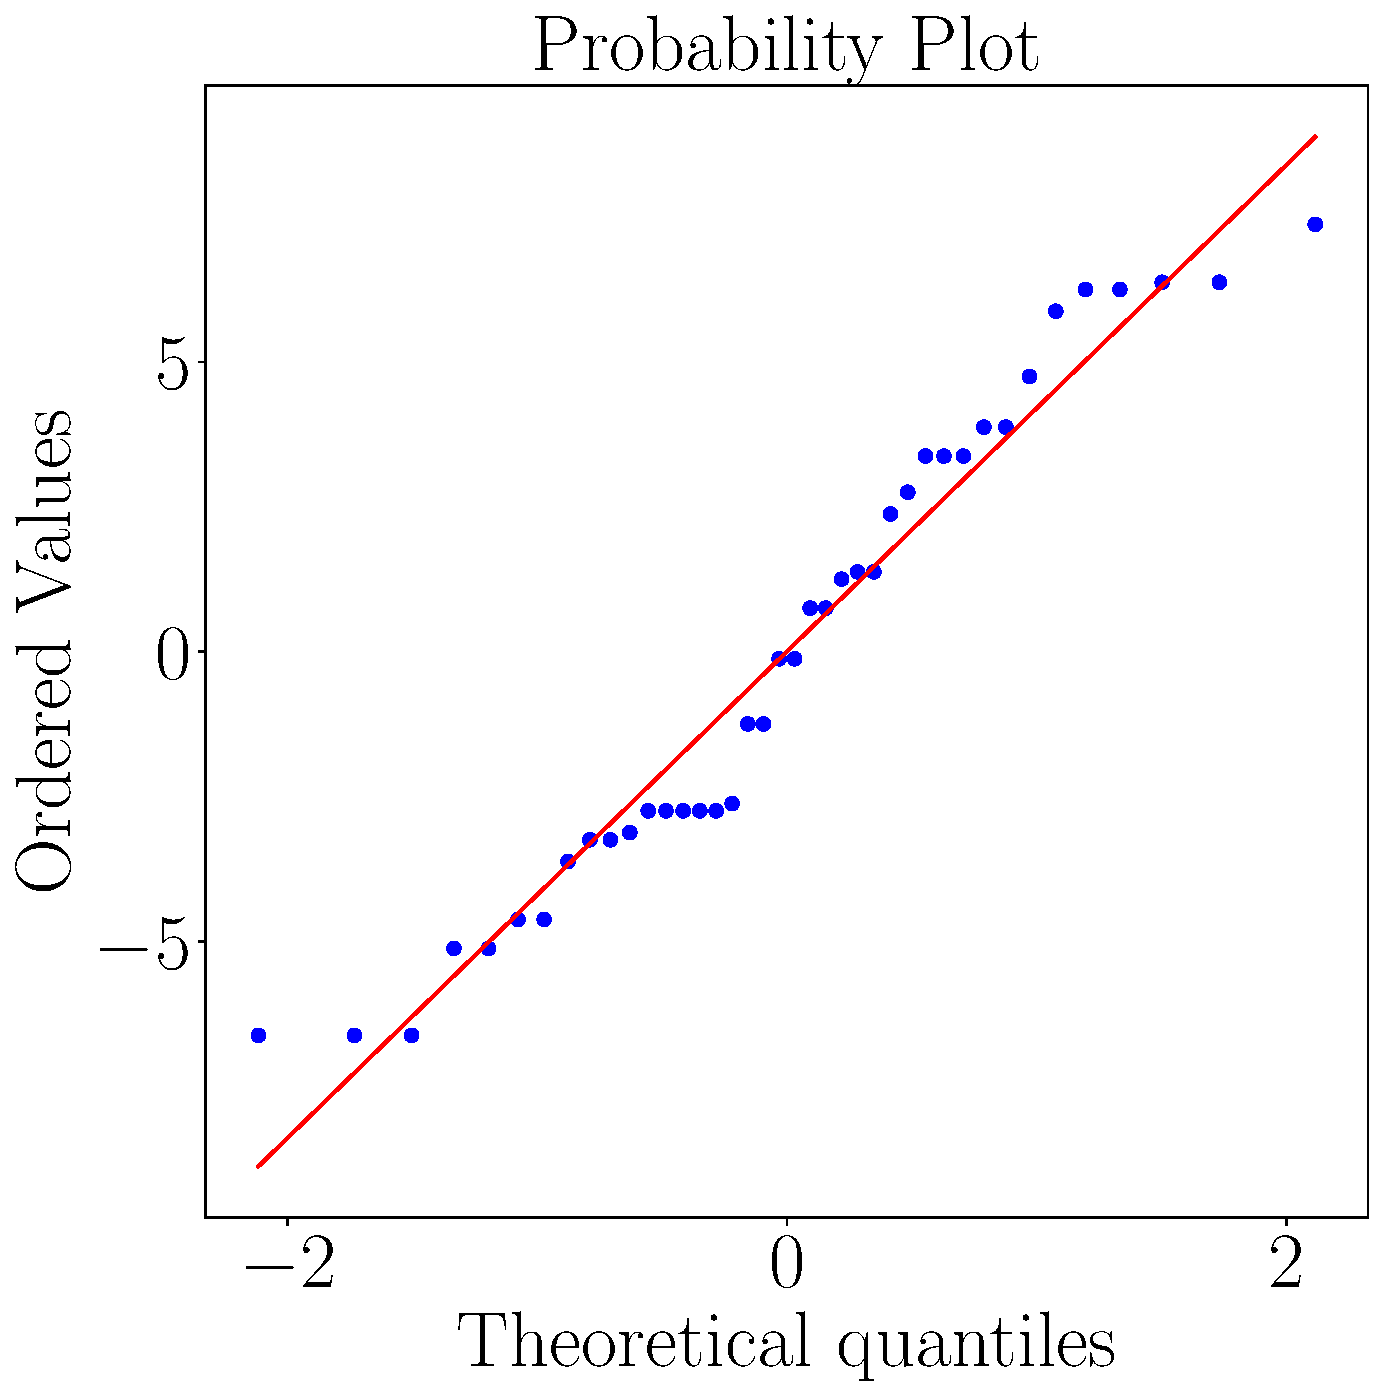
\includegraphics[width = \textwidth]{Resultados/Nasa/Figuras/pdf/qqplot_md_avg_two_way_blind.pdf}
        \caption{QQ plot of the mental demand of the blind participants on each method.}
        \label{fig:qqplot_md_avg_two_way_blind}
    \end{minipage}
    \begin{minipage}{0.075\textwidth}
        \hfill
    \end{minipage}
    \begin{minipage}{0.45\textwidth}
        \centering
        %\vspace{1ex}
        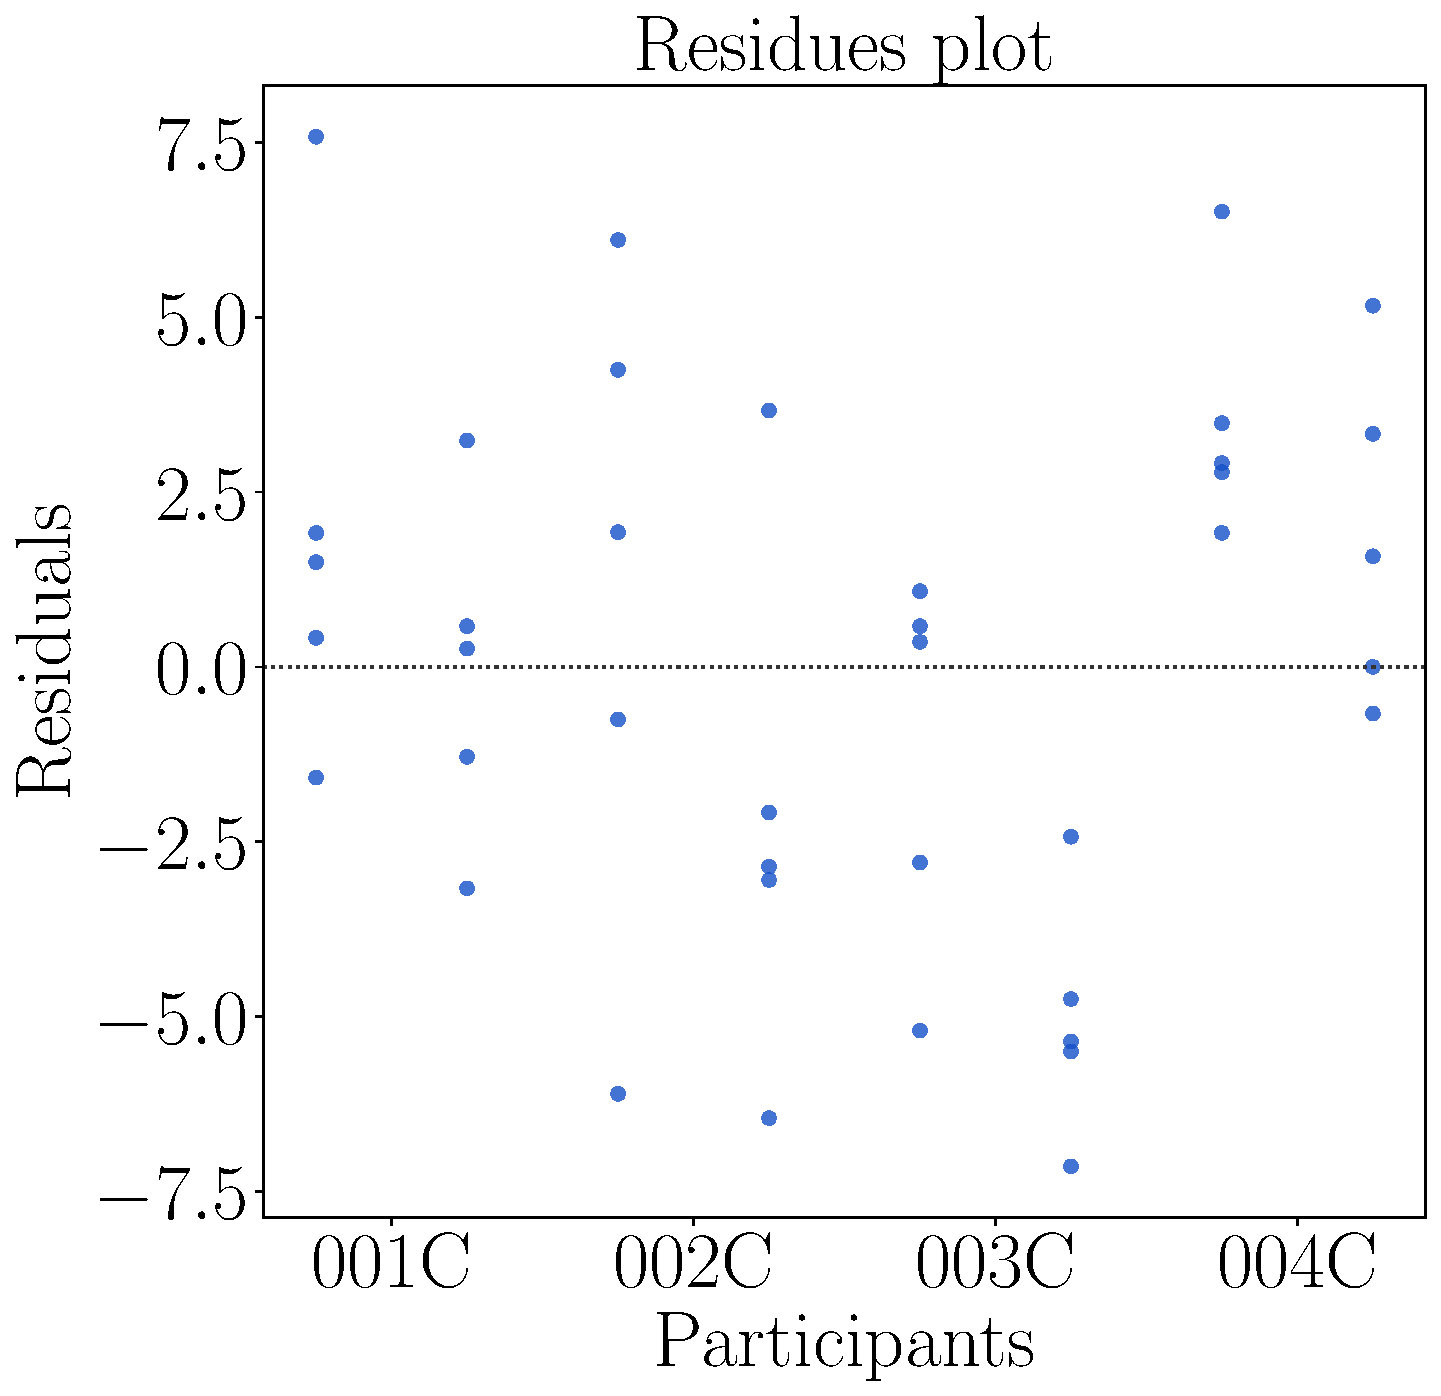
\includegraphics[width = \textwidth]{Resultados/Nasa/Figuras/pdf/residplot_md_avg_two_way_blind.pdf}
        \caption{Residual plot of the mental demand score the blind participants on each method.}
        \label{fig:residplot_md_avg_two_way_blind}
    \end{minipage}
\end{figure}

Following, the statistical model of Equation 5.1 is used for the analysis of variance (ANOVA): 

\begin{equation}
    \label{eq:statistical_model}
    y_{ijk} = \mu + \tau_i + \beta_j + \msout{\omega_k} + (\tau\beta_{ij}) + e
\end{equation}

where:

\begin{itemize}
    \item $y_{ij}$ - output variable for method $i$, round $j$ and participant $k$;
    \item $\mu$ - mean of all the observations;
    \item $\tau_i$ - variance from method $i$;
    \item $\beta_j$ - variance from round $j$;
    \item \sout{$\omega_k$} - variance from participant k, which is treated as a block;
    \item $\tau\beta_{ij}$ - combined variance from the interaction between method i and round j;
    \item $e$ - residual error.
\end{itemize}

The results of ANOVA are presented in Table \ref{tab:blocanova_md_avg_two_way_blind}. ANOVA tests the hypothesis that the means of independent data groups are equal or not. In the literature, a p-value of 0.05 is commonly adopted as a threshold to confirm the hypothesis. A p-value < 0.05 indicates that the means of the groups are statistically different with 95\% of confidence. According to this criterion, neither method or round have a significant influence on the mental demand.

However, due to the low number of participants, the threshold of 0.1 could also be considered. In this case, it indicates, with 90\% confidence, that the mean of the "first" and "return" rounds are different. For the guidance method, the p-value of 0.170 is close to the threshold but slightly higher, suggesting that the means may be different. However, this hypothesis is not statistically confirmed with the current data. 


\begin{table}[!htb]
\centering
\caption{Anova p-value for the mental demand average on each method for blinded users.}
\label{tab:blocanova_md_avg_two_way_blind}
\begin{tabular}{lrrrrl}
\toprule
               Source &  Squared sum &  DOF & Squared average &     F & \begin{tabular}[c]{@{}l@{}}P-Value \\ $(F_{0} > F)$\end{tabular} \\
\midrule
Participants (Blocks) &      298.475 &    3 &          99.492 & 8.133 &                                                                  \\
         \    Methods &       85.150 &    4 &          21.288 & 1.740 &                                                            0.170 \\
          \    Rounds &       42.025 &    1 &          42.025 & 3.436 &                                                            0.075 \\
     \    Interaction &        2.850 &    4 &           0.712 & 0.058 &                                                            0.993 \\
   Experimental Error &      330.275 &   27 &          12.232 &       &                                                                  \\
                Total &      758.775 &   39 &                 &       &                                                                  \\
\bottomrule
\end{tabular}
\end{table}



In order to conclude the analysis of the NASA-TLX mental demand, Table \ref{tab:md_var_average_group_blind} brings the average difference between the mental demand of the "first" and "return" rounds. Unexpectedly, it shows that the most significant variation is obtained to the "base", i.e., the guidance method the participant uses and, therefore, should not present a significant variation. The methods with the lower variation was "audio", probably because it already had a shallow score in the first round. 


\begin{table}[!htb]
\centering
\caption{Mental demand variation grouped by participant and visual condition}
\label{tab:md_var_average_group_blind}
\begin{tabular}{lrrrrrr}
\toprule
{} &  Base & Audio & \begin{tabular}[c]{@{}l@{}}Haptic\\ Belt\end{tabular} & \begin{tabular}[c]{@{}l@{}}Virtual\\ Cane\end{tabular} & Mixture \\
Visual Condition &       &       &                                                       &                                                        &         \\
\midrule
Blind            &  -2.5 &  -1.0 &                                                  -2.2 &                                                   -2.2 &    -2.2 \\
\bottomrule
\end{tabular}
\end{table}



\FloatBarrier

%%%%%%%%%%%%%%%%%%%%%%%%%%%%%%%%%%%%%%%%%%%%%%%%%%%%%%%%%%%%%%%%%%%%%%%%%%%
%%%%%%%%%%%%%%%%%%%%%%%%%%%%%%%%%%%%%%%%%%%%%%%%%%%%%%%%%%%%%%%%%%%%%%%%%%%
%%%%%%%%%%%%%%%%%%%%%%%%%%%%%%%%%%%%%%%%%%%%%%%%%%%%%%%%%%%%%%%%%%%%%%%%%%%
%%%%%%%%%%%%%%%%%%%%%%%%%%%%%%%%%%%%%%%%%%%%%%%%%%%%%%%%%%%%%%%%%%%%%%%%%%%


\paragraph{Analysis of the NASA-TLX score}\mbox{}\\

This section repeats the analysis steps of the previous section but now considers the mean value of all dimensions of NASA-TLX, referred to in this text as the global score. Table \ref{tab:nasa_table_blind} presents the global score of each blind participant. 


\begin{table}[!htb]
\centering
\caption{NASA-TLX score felled by the blinded participants.}
\label{tab:nasa_table_blind}
\begin{tabular}{llrrrrr}
\toprule
     &        &  Base &  Audio & \begin{tabular}[c]{@{}l@{}}Haptic\\ Belt\end{tabular} & \begin{tabular}[c]{@{}l@{}}Virtual\\ Cane\end{tabular} & Mixture \\
Participant & Round &       &        &                                                       &                                                        &         \\
\midrule
001C & First & 4.833 &  4.000 &                                                 8.833 &                                                  5.167 &   6.333 \\
     & Return & 4.167 &  4.000 &                                                 6.667 &                                                  4.500 &   6.167 \\
002C & First & 6.333 &  4.833 &                                                 4.833 &                                                  9.000 &   7.000 \\
     & Return & 4.500 &  4.833 &                                                 4.833 &                                                  7.000 &   5.167 \\
003C & First & 4.000 &  4.000 &                                                 5.333 &                                                  6.667 &   3.500 \\
     & Return & 4.000 &  3.833 &                                                 3.667 &                                                  3.500 &   3.500 \\
004C & First & 9.833 & 10.000 &                                                12.667 &                                                  9.667 &  11.000 \\
     & Return & 8.667 &  9.167 &                                                11.667 &                                                  9.333 &  10.833 \\
\bottomrule
\end{tabular}
\end{table}



Figure \ref{fig:barplot_nasa_avg_5_scene_blind} brings the corresponding barplot with the mean value and standard deviation for each guidance method and each round. In a qualitative comparison with Figure \ref{fig:barplot_md_avg_5_scene_blind}, the differences between the methods are confirmed but softened. It is possible to notice that the mean score of "audio" and "base" are still lower than that of the other methods. The differences between "first" and "return" rounds are also reduced. However, the standard deviation is also considerably reduced for all methods, and especially for the haptic belt.

\begin{figure}[!htb]
    \centering
    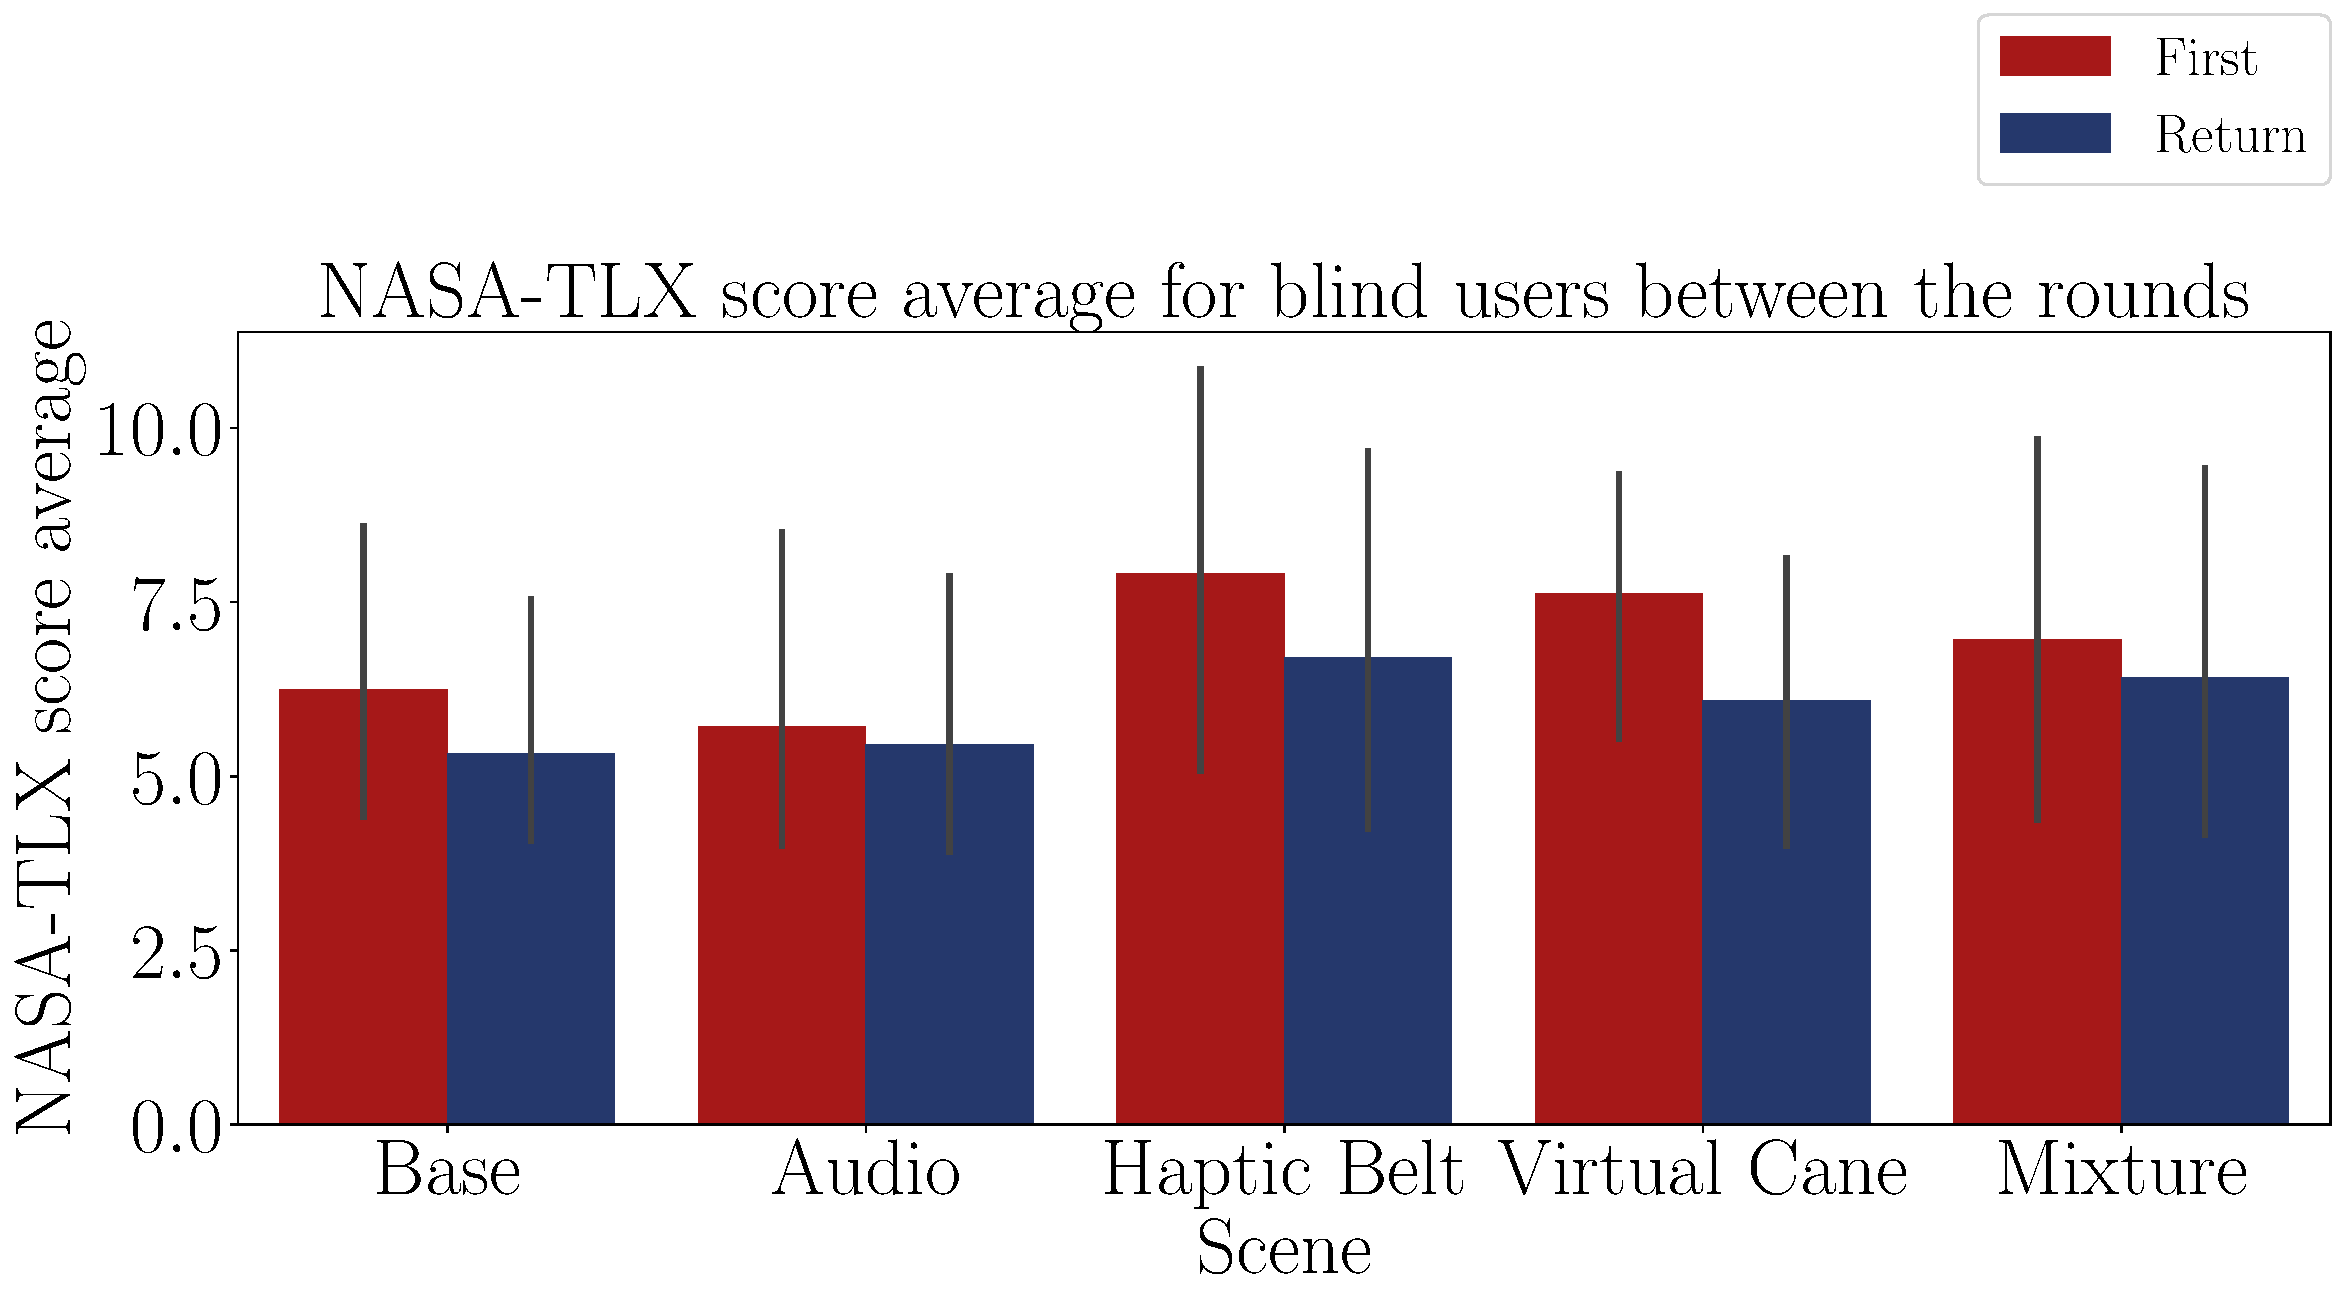
\includegraphics[width = \textwidth]{Resultados/Nasa/Figuras/pdf/barplot_nasa_avg_5_scene_blind.pdf}
    \caption{Barplot of the average NASA-TLX score of the blind participants on each method.}
    \label{fig:barplot_nasa_avg_5_scene_blind}
\end{figure}

Figure \ref{fig:boxplot_nasa_blind_scene} presents the boxplot with the NASA-TLX global score grouped by the methods. Similar to what happened for the "mental demand", it is possible to split the methods into two different groups: "base" and "audio", which require a lower level of workload, and another group, which requires a higher level. Figure \ref{fig:boxplot_nasa_blind_rounds} presents a boxplot with the NASA-TLX global score grouped by the rounds, showing that the two groups are still different. 

\begin{figure}[!htb]
    \centering
    \begin{minipage}{0.45\textwidth}
        \centering
        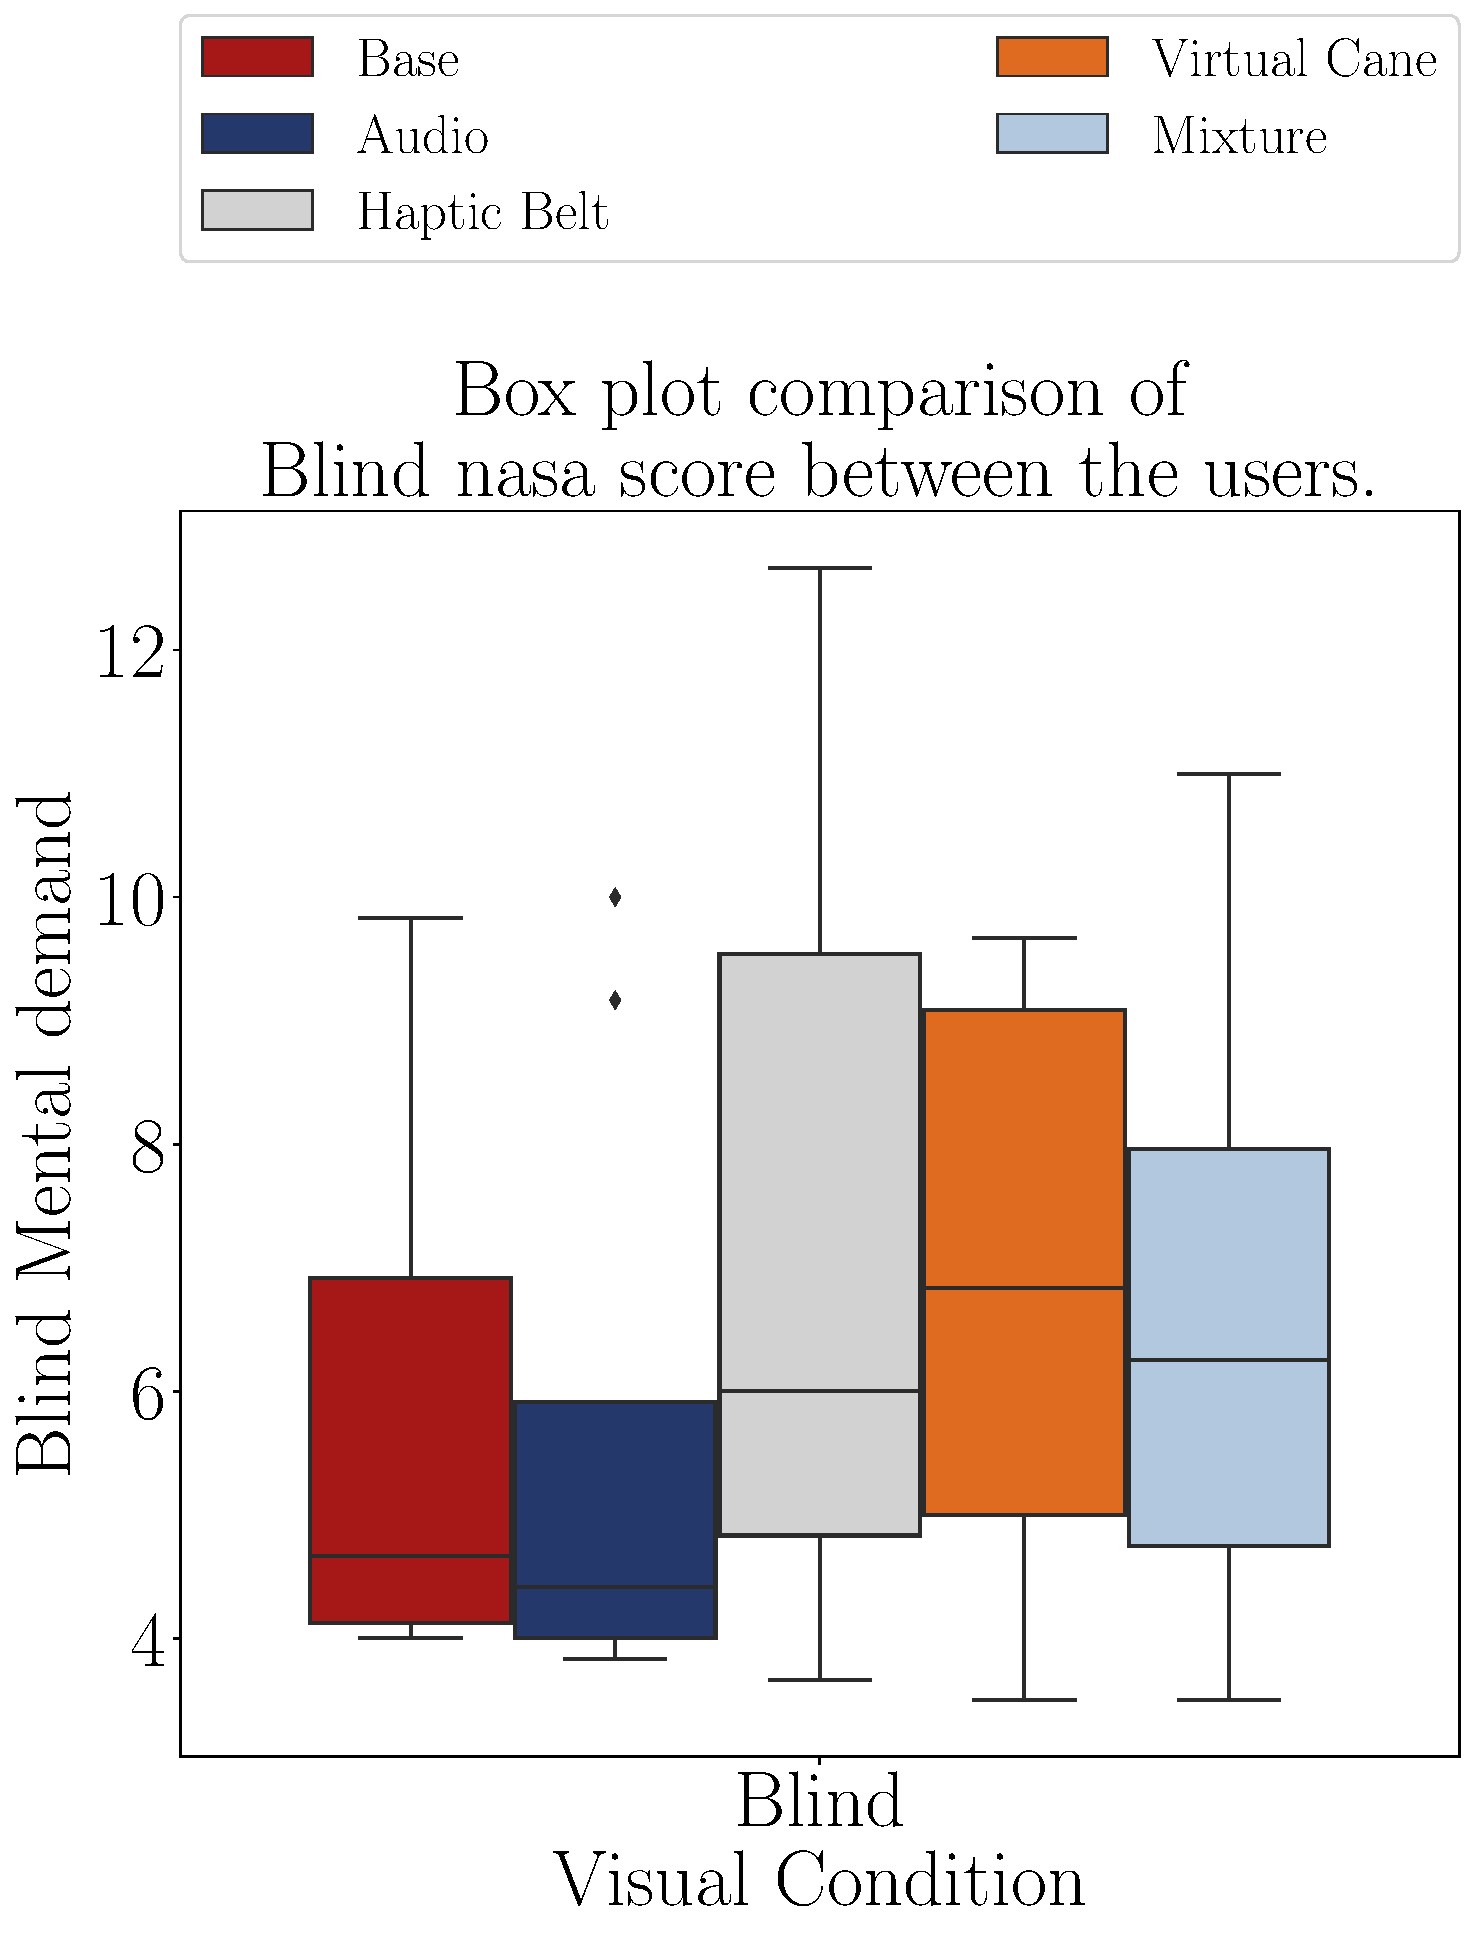
\includegraphics[width = \textwidth]{Resultados/Nasa/Figuras/pdf/boxplot_nasa_blind_scene.pdf}
        \caption{Boxplot of the NASA-TLX of the blind participants grouped by the methods.}
        \label{fig:boxplot_nasa_blind_scene}
    \end{minipage}
    \begin{minipage}{0.075\textwidth}
        \hfill
    \end{minipage}
    \begin{minipage}{0.45\textwidth}
        \centering
        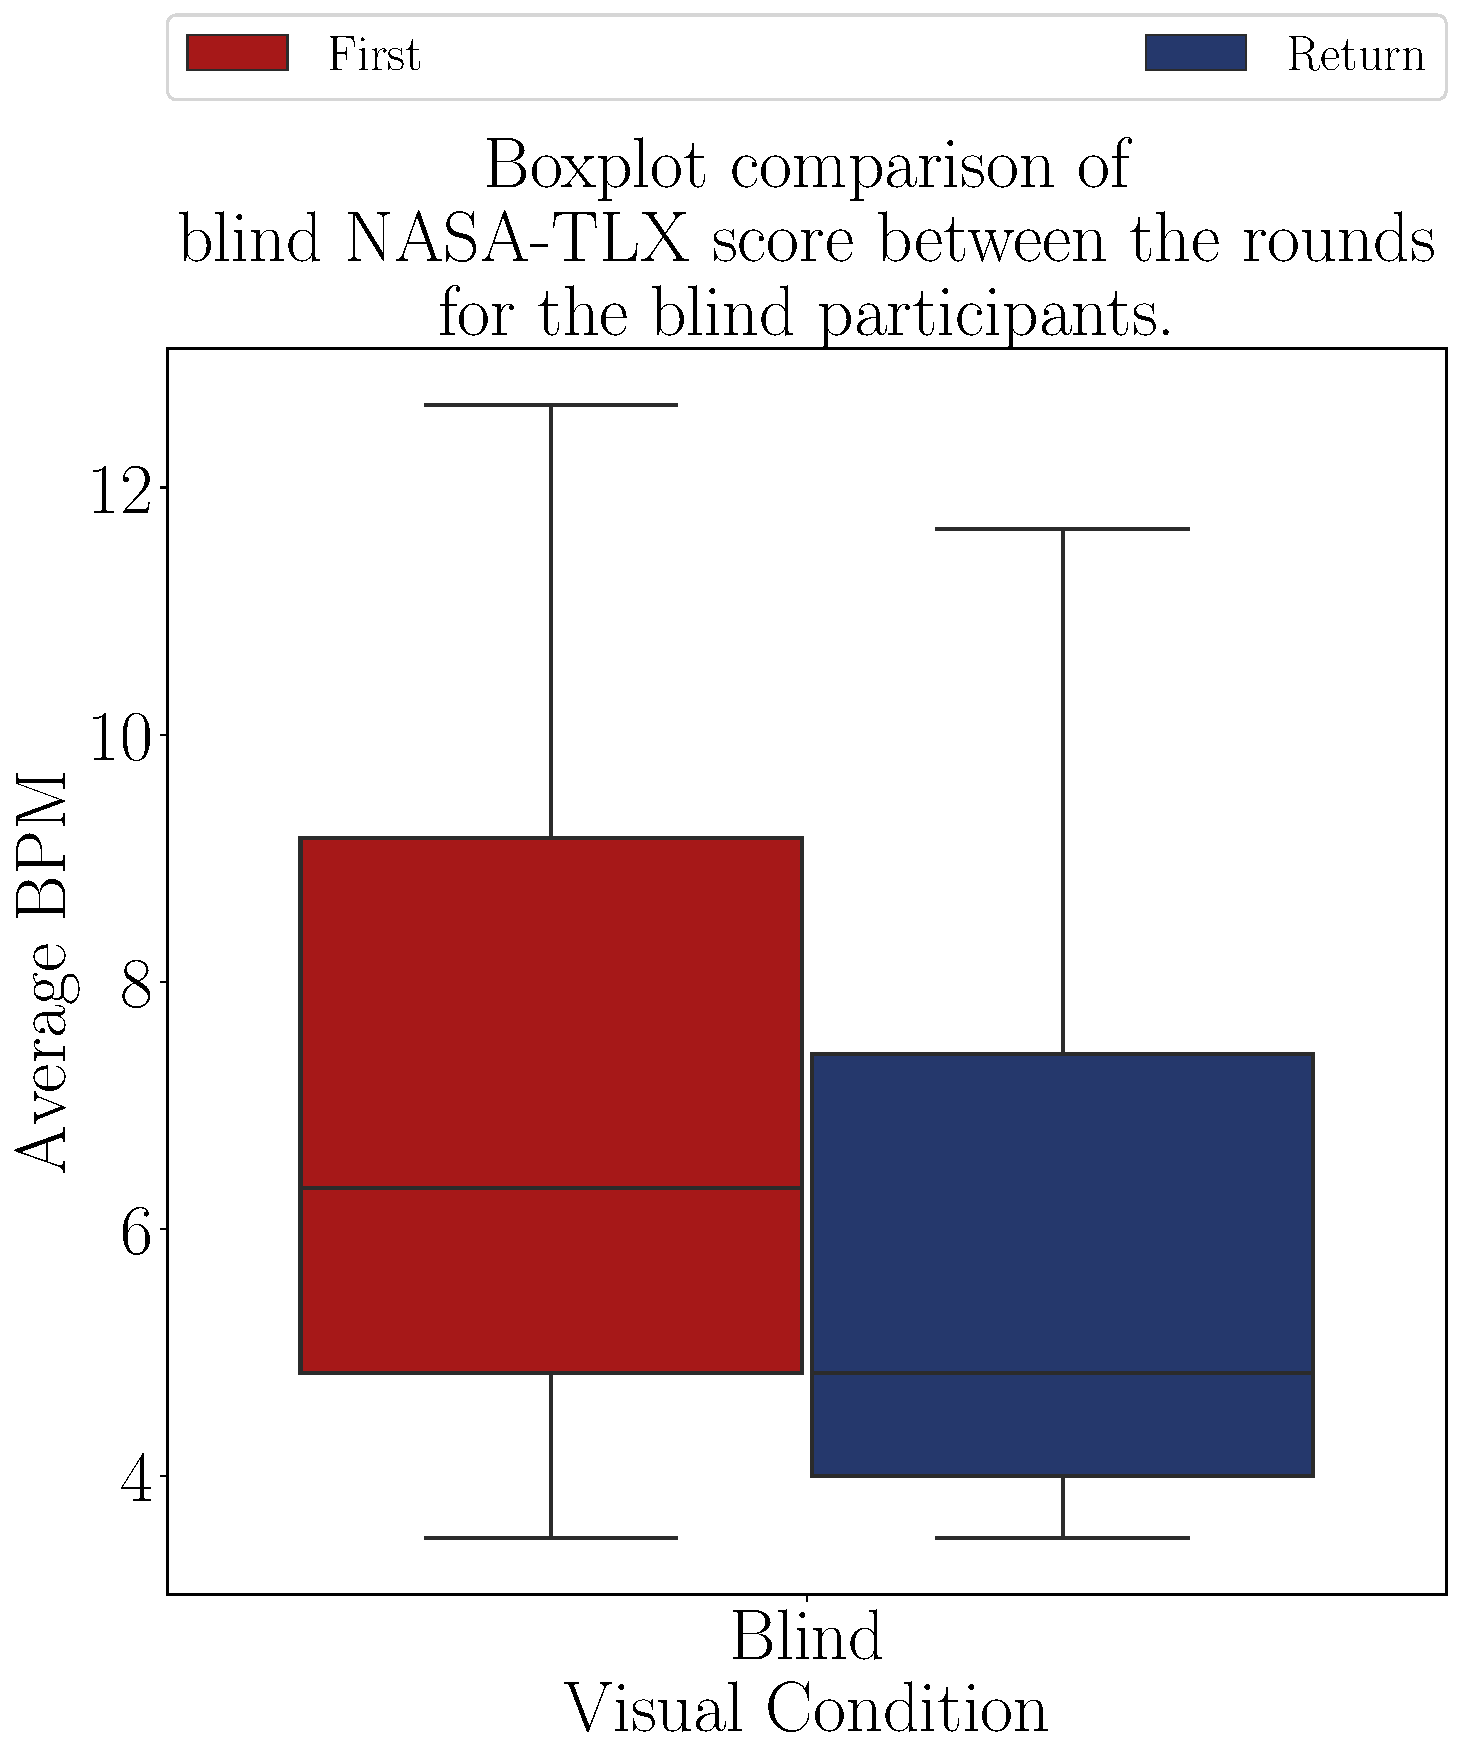
\includegraphics[width = \textwidth]{Resultados/Nasa/Figuras/pdf/boxplot_nasa_blind_rounds.pdf}
        \caption{Boxplot of the NASA-TLX demand of the blind participants grouped by the round.}
        \label{fig:boxplot_nasa_blind_rounds}
    \end{minipage}
\end{figure}

Figures \ref{fig:qqplot_nasa_avg_two_way_blind} and \ref{fig:residplot_nasa_avg_two_way_blind} presents the QQ plot and residual distribution of the NASA-TLX global score, showing that the data are normally distributed. However, the residuals are not so homogeneous as in the previous case, showing that the participants have different variability among them.

\begin{figure}[!htb]
    \centering
    \begin{minipage}{0.45\textwidth}
        \centering
        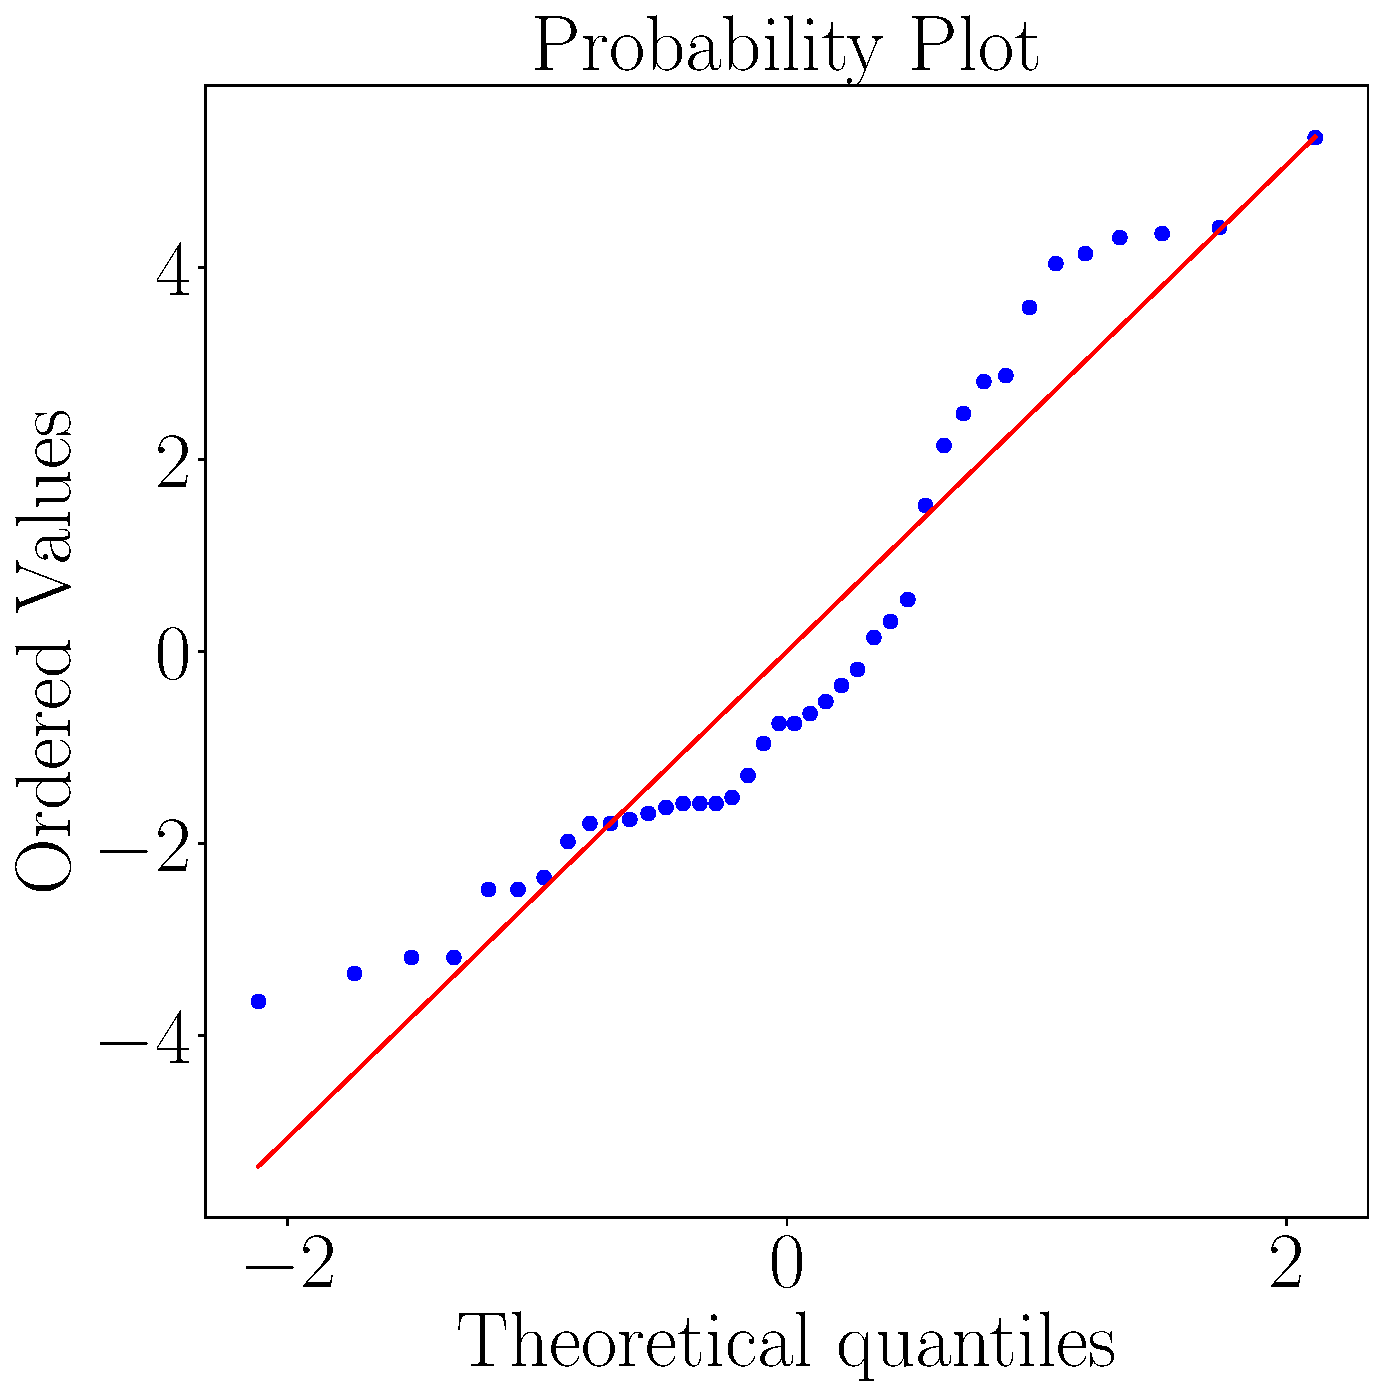
\includegraphics[width = \textwidth]{Resultados/Nasa/Figuras/pdf/qqplot_nasa_avg_two_way_blind.pdf}
        \caption{QQ plot of the NASA-TLX score of the blind participants on each method.}
        \label{fig:qqplot_nasa_avg_two_way_blind}
    \end{minipage}
    \begin{minipage}{0.075\textwidth}
        \hfill
    \end{minipage}
    \begin{minipage}{0.45\textwidth}
        %\vspace{2ex}
        \centering
        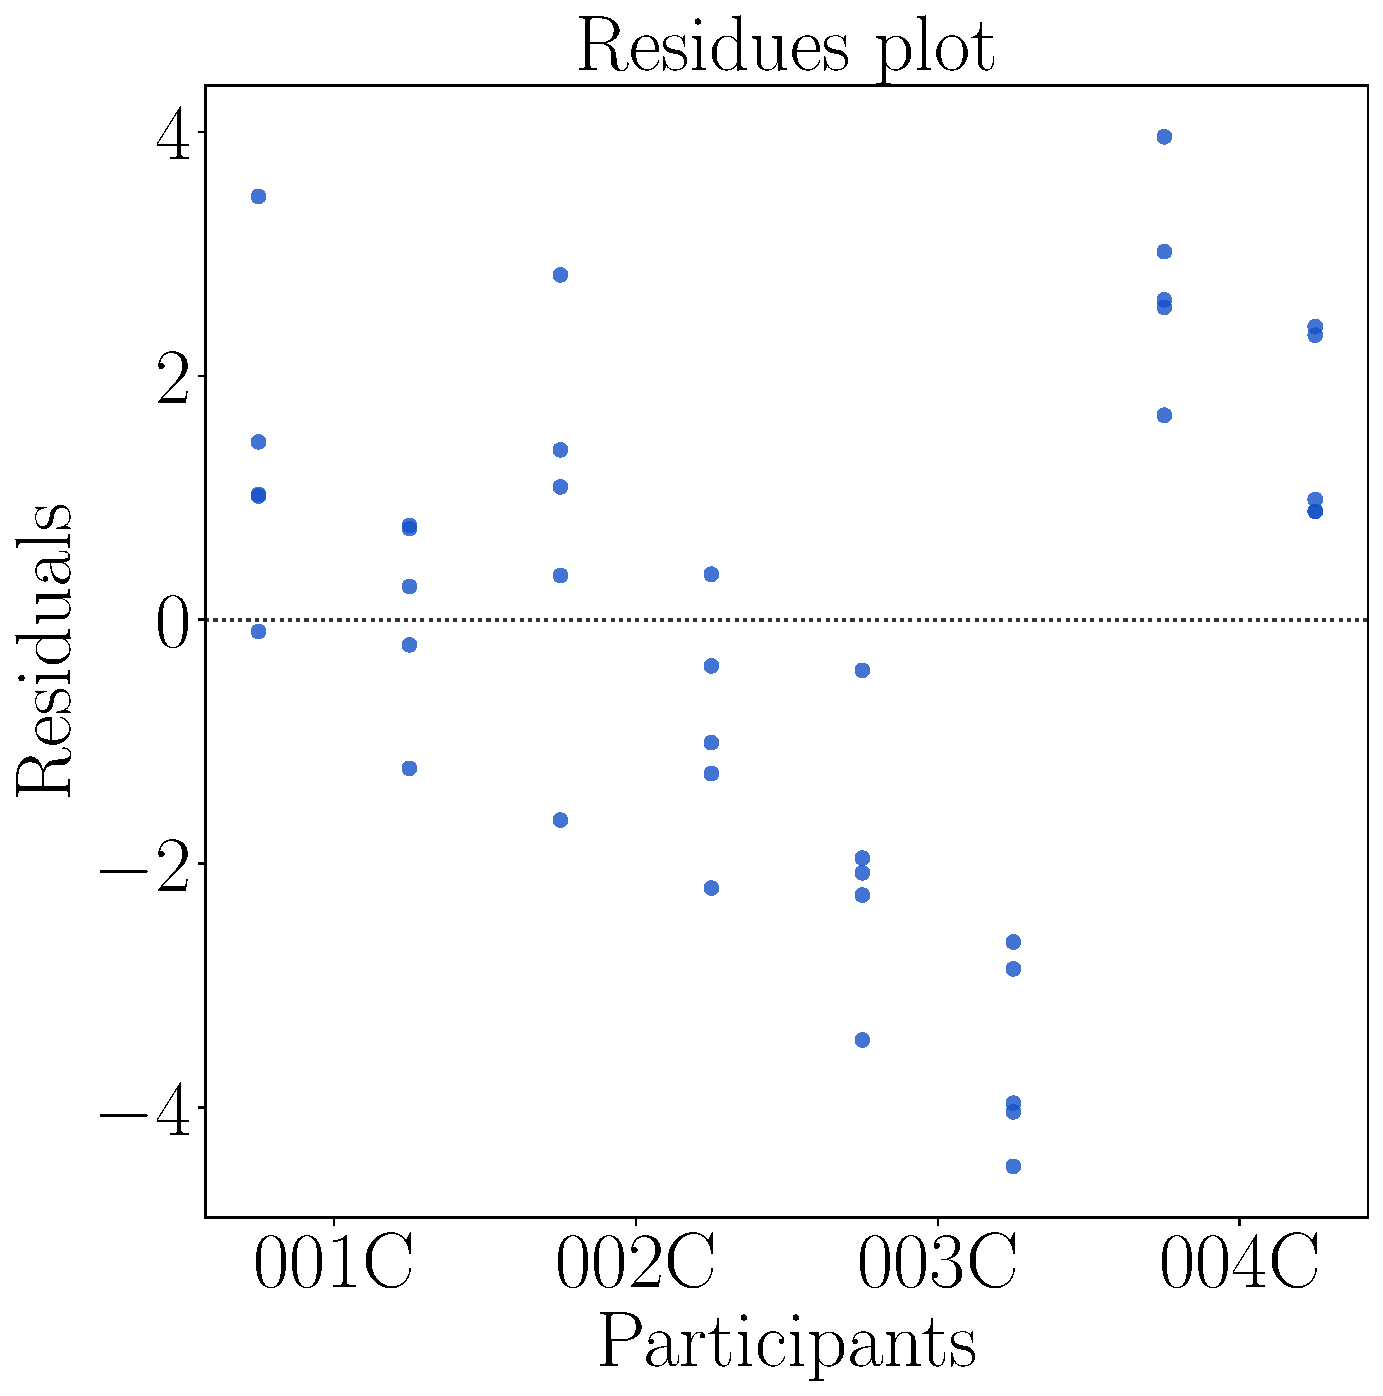
\includegraphics[width = \textwidth]{Resultados/Nasa/Figuras/pdf/residplot_nasa_avg_two_way_blind.pdf}
        \caption{Residual plot of the NASA-TLX score the blind participants on each method.}
        \label{fig:residplot_nasa_avg_two_way_blind}
    \end{minipage}
\end{figure}

Table \ref{tab:blocanova_nasa_avg_two_way_blind} brings the p-value resulting from ANOVA. In this case, both the methods and the rounds were appointed as significant variables that influence the mean value of the NASA-TLX global score. 


\begin{table}[!htb]
\centering
\caption{Anova p-value for the NASA-TLX score on each method for blinded users.}
\label{tab:blocanova_nasa_avg_two_way_blind}
\begin{tabular}{lrrrrl}
\toprule
          Source & P-Value \\
\midrule
    \    Methods & 0.029** \\
     \    Rounds & 0.022** \\
\    Interaction &   0.814 \\
\bottomrule
\end{tabular}
\end{table}



Finally, Table \ref{tab:lsd_nasa_avg_two_way_blind} presents the results of a pairwise Fisher LSD test comparing each pair of guidance methods. The results show that only "audio" is similar "base". All the other methods are different from each other.


\begin{table}[!htb]
\centering
\caption{Cross validation p-value for the NASA-TLX score on each method for blinded users.}
\label{tab:lsd_nasa_avg_two_way_blind}
\begin{tabular}{rclr}
\toprule
      \multicolumn{3}{c}{Method} &                                           Analysis \\
\midrule
              Base & $X$ & Audio &                   $H_0 : \mu_{Base} = \mu_{Audio}$ \\
        Base & $X$ & Haptic Belt &         $H_1 : \mu_{Base} \ne \mu_{Haptic Belt}**$ \\
       Base & $X$ & Virtual Cane &        $H_1 : \mu_{Base} \ne \mu_{Virtual Cane}**$ \\
            Base & $X$ & Mixture &             $H_1 : \mu_{Base} \ne \mu_{Mixture}**$ \\
       Audio & $X$ & Haptic Belt &        $H_1 : \mu_{Audio} \ne \mu_{Haptic Belt}**$ \\
      Audio & $X$ & Virtual Cane &       $H_1 : \mu_{Audio} \ne \mu_{Virtual Cane}**$ \\
           Audio & $X$ & Mixture &            $H_1 : \mu_{Audio} \ne \mu_{Mixture}**$ \\
Haptic Belt & $X$ & Virtual Cane & $H_1 : \mu_{Haptic Belt} \ne \mu_{Virtual Cane}**$ \\
     Haptic Belt & $X$ & Mixture &      $H_1 : \mu_{Haptic Belt} \ne \mu_{Mixture}**$ \\
    Virtual Cane & $X$ & Mixture &         $H_0 : \mu_{Virtual Cane} = \mu_{Mixture}$ \\
\bottomrule
\end{tabular}
\end{table}



Table \ref{tab:nasa_var_group_blind} shows the difference in the NASA-TLX global score between the first and return rounds. It shows that the "audio" difference is the lowest among all methods, while the highest difference is for the "virtual cane".


\begin{table}[!htb]
\centering
\caption{NASA-TLX score grouped by participant and visual Condition.}
\label{tab:nasa_var_group_blind}
\begin{tabular}{lrrrrrr}
\toprule
{} &   Base &  Audio & \begin{tabular}[c]{@{}l@{}}Haptic\\ Belt\end{tabular} & \begin{tabular}[c]{@{}l@{}}Virtual\\ Cane\end{tabular} & Mixture \\
Visual Condition &        &        &                                                       &                                                        &         \\
\midrule
Blind            &  -0.92 &  -0.25 &                                                 -1.21 &                                                  -1.54 &   -0.54 \\
\bottomrule
\end{tabular}
\end{table}



\FloatBarrier

\subsubsection{Adapted SAGAT}
\label{subsubsec:results_adapted_sagat_1}

In this subsection, the SAGAT questionnaire is analyzed. Its result may give an idea of the mental map the participant is drawing. For each question a participant could score 1 point or a fraction of it. The total score of each blind participant is presented on the Table \ref{tab:sagat_table_blind} and they are plotted in the Figures \ref{fig:barplot_sagat_avg_5_scene_blind}, where it is visually noticeable that the performance better the second time they visit the room. 


\begin{table}[!htb]
\centering
\caption{SAGAT global score felled by the blinded participants.}
\label{tab:sagat_table_blind}
\begin{tabular}{llrrrrr}
\toprule
     &        &   Base &  Audio & \begin{tabular}[c]{@{}l@{}}Haptic\\ Belt\end{tabular} & \begin{tabular}[c]{@{}l@{}}Virtual\\ Cane\end{tabular} & Mixture \\
Participant & Round &        &        &                                                       &                                                        &         \\
\midrule
001C & First &   6.25 &   5.50 &                                                  5.33 &                                                   5.83 &   3.500 \\
     & Return &   6.25 &   6.50 &                                                  8.50 &                                                   5.50 &   5.500 \\
002C & First &   6.75 &   4.50 &                                                  3.99 &                                                   4.50 &   6.250 \\
     & Return &   5.25 &   5.00 &                                                  4.00 &                                                   6.50 &   8.500 \\
003C & First &   7.25 &   7.50 &                                                  7.49 &                                                   4.66 &   9.000 \\
     & Return &  10.00 &  10.00 &                                                  8.50 &                                                   9.00 &   9.000 \\
004C & First &   7.50 &   6.00 &                                                  7.66 &                                                   4.99 &   6.500 \\
     & Return &   9.00 &   6.00 &                                                  9.25 &                                                   7.25 &   9.000 \\
\bottomrule
\end{tabular}
\end{table}



\begin{figure}[!htb]
    \centering
    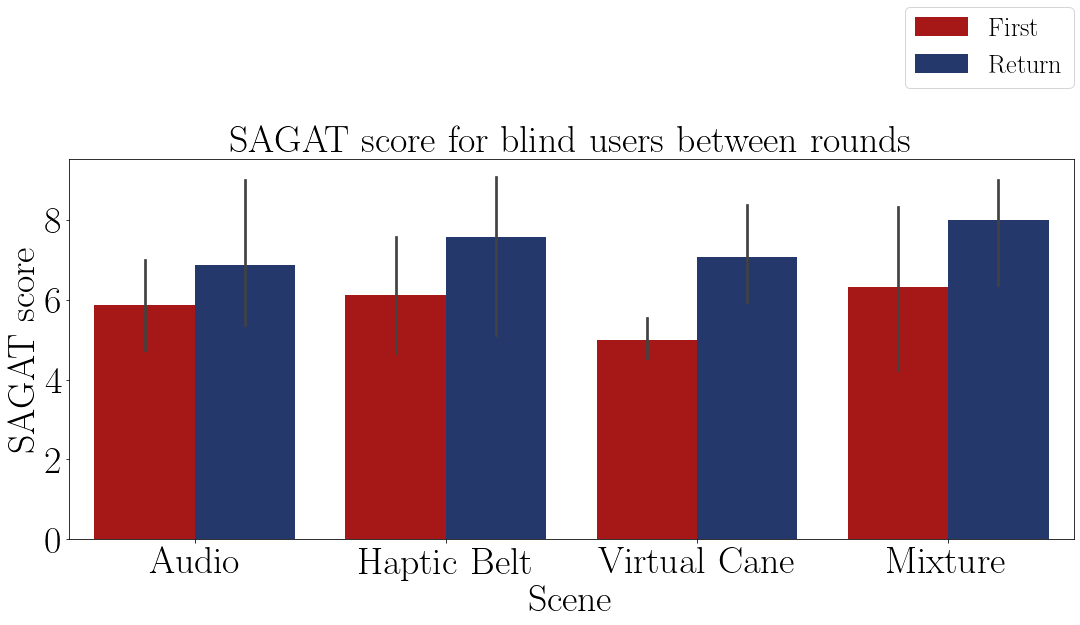
\includegraphics[width = 0.8\linewidth]{Resultados/Sagat/Figuras/png/barplot_sagat_avg_5_scene_blind.png}
    \caption{Barplot of the average SAGAT score of the blind participants on each method.}
    \label{fig:barplot_sagat_avg_5_scene_blind}
\end{figure}

The boxplot in the Figure \ref{fig:boxplot_sagat_blind_scene} shows that there are two groups of scores one with the “Base”, “Haptic Belt” and the “Mixture” methods, and the second group with the “Audio” and the “Virtual Cane” methods. The first group scored higher than the second one. The Figure \ref{fig:boxplot_sagat_blind_rounds} shows a noticible difference between the scores when grouped by their corresponding round.

\begin{figure}[!htb]
    \centering
    \begin{minipage}{0.45\textwidth}
        \centering
        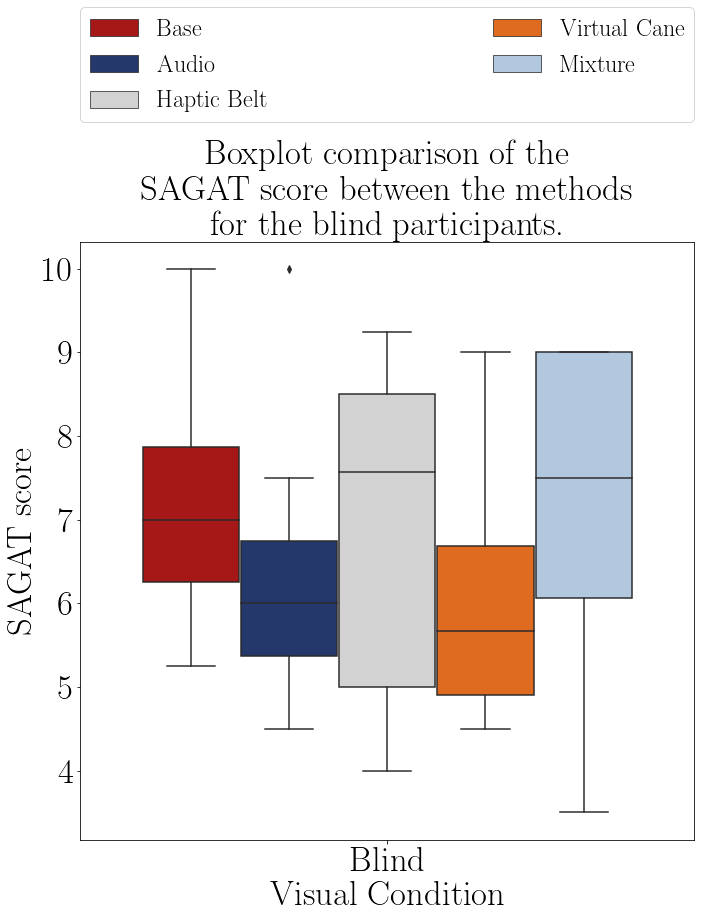
\includegraphics[width = 0.8\linewidth]{Resultados/Sagat/Figuras/png/boxplot_sagat_blind_scene.png}
        \caption{Boxplot of the SAGAT score of the blind participants grouped by method.}
        \label{fig:boxplot_sagat_blind_scene}
    \end{minipage}
    \begin{minipage}{0.45\textwidth}
        \centering
        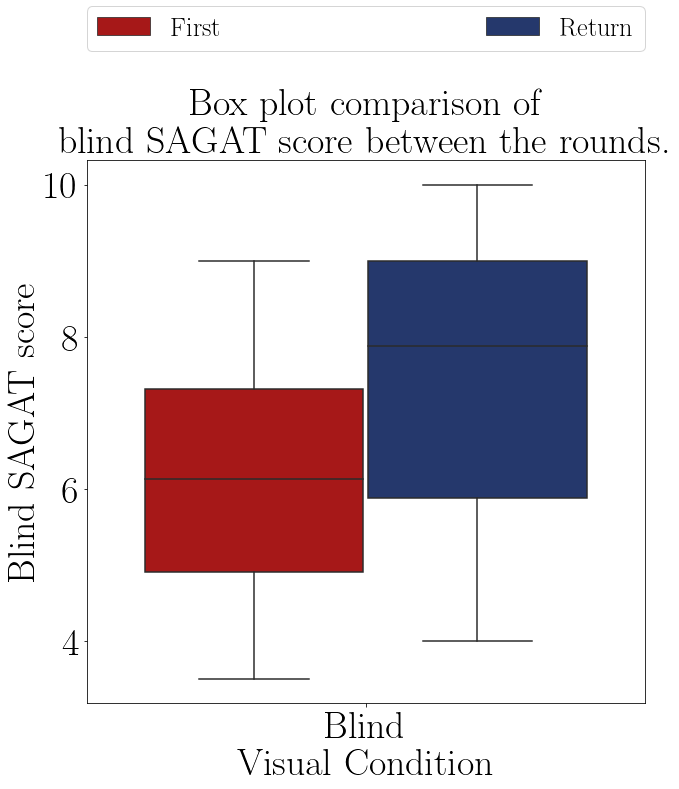
\includegraphics[width = 0.8\linewidth]{Resultados/Sagat/Figuras/png/boxplot_sagat_blind_rounds.png}
        \caption{Boxplot of the SAGAT score of the blind participants grouped by round.}
        \label{fig:boxplot_sagat_blind_rounds}
    \end{minipage}
\end{figure}

The Table \ref{tab:sagat_average_group_blind} shows the average SAGAT score in the “blind” sample and is possible to notice how the average score by the “blind” sample was lower during the “Audio” and the “Base” methods.


\begin{table}[!htb]
\centering
\caption{SAGAT score average grouped by participant and visual condition}
\label{tab:sagat_average_group_blind}
\begin{tabular}{lrrrrrr}
\toprule
{} &  Base & Audio & \begin{tabular}[c]{@{}l@{}}Haptic\\ Belt\end{tabular} & \begin{tabular}[c]{@{}l@{}}Virtual\\ Cane\end{tabular} &  Mixture \\
Visual Condition &       &       &                                                       &                                                        &          \\
\midrule
Blind            &  7.28 &  6.38 &                                                  6.84 &                                                   6.03 &    7.156 \\
\bottomrule
\end{tabular}
\end{table}




The Figures \ref{fig:qqplot_sagat_avg_two_way_blind} and \ref{fig:residplot_sagat_avg_two_way_blind} shows the distribution and variance of the Table \ref{tab:sagat_table_blind}. These Figures shows that the data are normally distributed and that the methods have a similar variance.
The Table \ref{tab:blocanova_sagat_avg_two_way_blind} shows the Anova test p-value of the SAGAT score of the "blind" sample. The round's p-values indicates that some have influence on the SAGAT score. Meaning that the participants did learn information about the room between the "First" and "Return" round. The method and the interaction between it and the round has no influence on the SAGAT score.


\begin{table}[!htb]
\centering
\caption{Anova p-value for the SAGAT score on each method for blinded users.}
\label{tab:blocanova_sagat_avg_two_way_blind}
\begin{tabular}{lrrrrr}
\toprule
               Source &  Squared sum &  DOF & Squared average &      F & \begin{tabular}[c]{@{}l@{}}P-Value \\ $(F_{0} > F)$\end{tabular} \\
\midrule
Participants (Blocks) &       48.231 &    3 &          16.077 &  9.731 &                                                                  \\
         \    Methods &        8.922 &    4 &           2.230 &  1.350 &                                                            0.277 \\
          \    Rounds &       18.975 &    1 &          18.975 & 11.485 &                                                          0.002** \\
     \    Interaction &        2.391 &    4 &           0.598 &  0.362 &                                                            0.834 \\
   Experimental Error &       44.608 &   27 &           1.652 &        &                                                                  \\
                Total &      123.127 &   39 &                 &        &                                                                  \\
\bottomrule
\end{tabular}
\end{table}



\begin{figure}[!htb]
    \centering
    \begin{minipage}{0.45\textwidth}
        \centering
        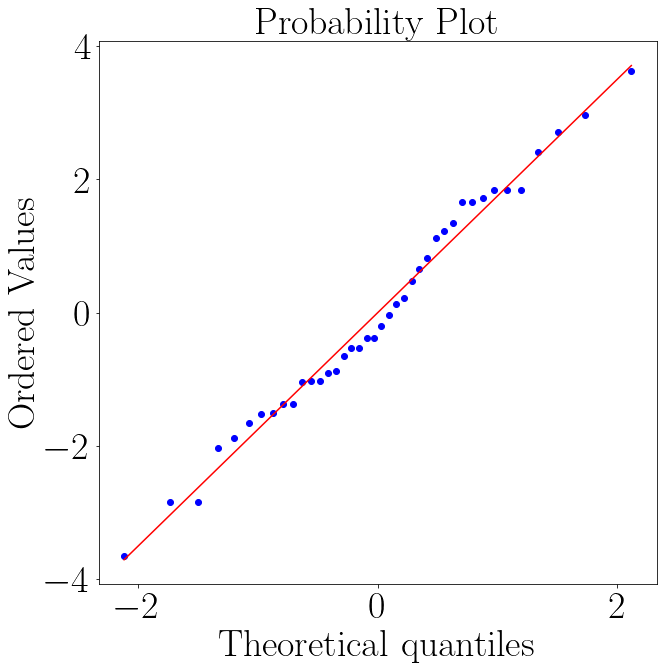
\includegraphics[width = 0.8\linewidth]{Resultados/Sagat/Figuras/png/qqplot_sagat_avg_two_way_blind.png}
        \caption{QQ plot of the SAGAT score of the blind participants on each method.}
        \label{fig:qqplot_sagat_avg_two_way_blind}
    \end{minipage}
    \begin{minipage}{0.45\textwidth}
        \centering
        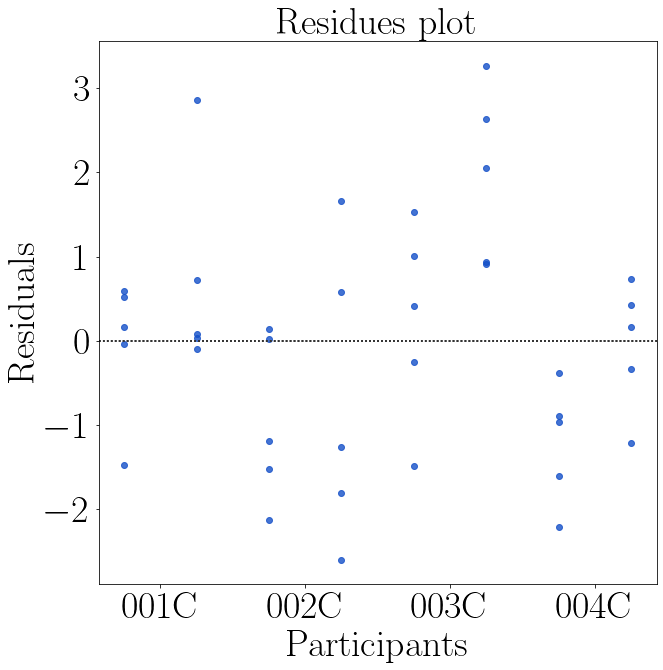
\includegraphics[width = 0.8\linewidth]{Resultados/Sagat/Figuras/png/residplot_sagat_avg_two_way_blind.png}
        \caption{Residual plot of the SAGAT score the blind participants on each method.}
        \label{fig:residplot_sagat_avg_two_way_blind}
    \end{minipage}
\end{figure}


%The Table \ref{tab:lsd_sagat_avg_two_way} presents the conclusion of a pairwise Fisher LSD test of the blind NASA-TLX score between all the guidance methods. The results show that only the "Audio" has a similar NASA-TLX score as the "Base" method, as it was also posible to notice at Figure \ref{fig:boxplot_sagat_blind_scene}.

%\input{Resultados/Sagat/Tabelas/lsd_sagat_avg_two_way}

The Table \ref{tab:sagat_var_group_blind} shows the average of the SAGAT score variation between the rounds. This table shows that the variation from the "Base" and the "Audio" was the lowest variation and the highest variation was the "Virtual Cane".


\begin{table}[!htb]
\centering
\caption{Adapted Sagat global score variation grouped by participant and visual Condition}
\label{tab:sagat_var_group_blind}
\begin{tabular}{lrrrrrr}
\toprule
{} &  Base &  Audio & \begin{tabular}[c]{@{}l@{}}Haptic\\ Belt\end{tabular} & \begin{tabular}[c]{@{}l@{}}Virtual\\ Cane\end{tabular} & Mixture \\
Visual Condition &       &        &                                                       &                                                        &         \\
\midrule
Blind            &  8.93 &  15.66 &                                                 23.49 &                                                  44.30 &   32.90 \\
\bottomrule
\end{tabular}
\end{table}



The Figures \ref{fig:qqplot_sagat_var_blind} and \ref{fig:residplot_sagat_var_blind} shows the distribution and variance of the SAGAT score variation of the Table \ref{tab:sagat_table_blind}. These Figures shows that the data are normally distributed and that the methods have a similar variance.
The Table \ref{tab:blocanova_sagat_var_blind} shows the Anova test p-value of the SAGAT score of the "blind" sample between the guidance methods. The p-value indicates that there are no difference between the variation in any method. 


\begin{table}[!htb]
\centering
\caption{Anova p-value for the SAGAT score variation on each method for blinded users.}
\label{tab:blocanova_sagat_var_blind}
\begin{tabular}{lrrrrr}
\toprule
               Source &  Squared sum &  DOF & Squared average &     F & \begin{tabular}[c]{@{}l@{}}P-Value \\ $(F_{0} > F)$\end{tabular} \\
\midrule
Participants (blocks) &     1176.902 &    3 &         782.885 & 0.473 &                                                                  \\
               Method &     3131.542 &    4 &         392.301 & 0.944 &                                                            0.472 \\
   Experimental error &     9956.458 &   12 &         829.705 &       &                                                                  \\
                Total &    14264.902 &   19 &                 &       &                                                                  \\
\bottomrule
\end{tabular}
\end{table}



\begin{figure}[!htb]
    \centering
    \begin{minipage}{0.45\textwidth}
        \centering
        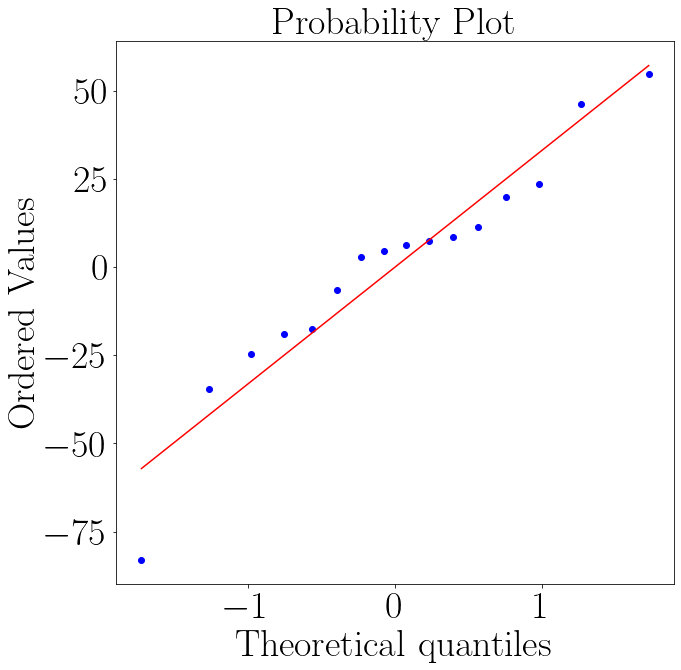
\includegraphics[width = 0.8\linewidth]{Resultados/Sagat/Figuras/png/qqplot_sagat_var_sight.png}
        \caption{QQ plot of the SAGAT score variation of the blind participants on each method.}
        \label{fig:qqplot_sagat_var_blind}
    \end{minipage}
    \begin{minipage}{0.45\textwidth}
        \centering
        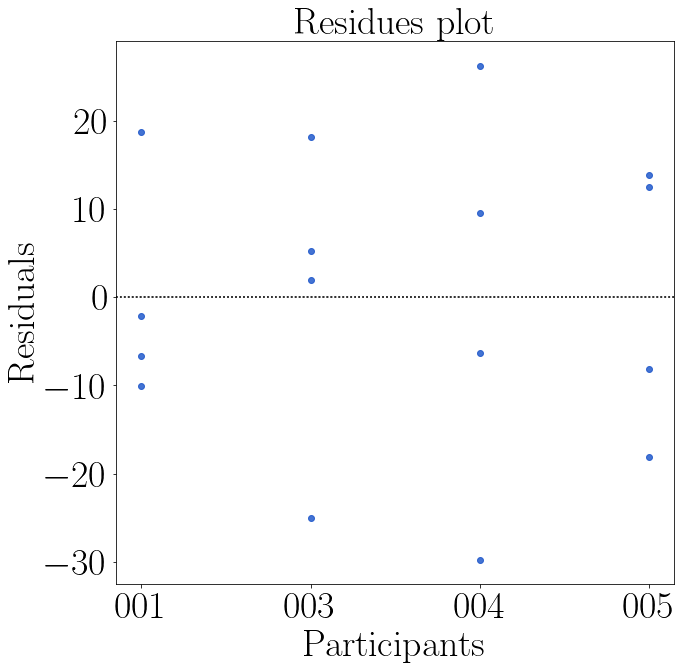
\includegraphics[width = 0.8\linewidth]{Resultados/Sagat/Figuras/png/residplot_sagat_var_sight.png}
        \caption{Residual plot of the SAGAT score variation of the blind participants on each method.}
        \label{fig:residplot_sagat_var_blind}
    \end{minipage}
\end{figure}

%The Table \ref{tab:lsdbloc_nasa_var} presents the conclusion of a pairwise Fisher LSD test of the blind NASA-TLX score between all the guidance methods. The results show that all methods have similar variations.

%
\begin{table}[!htb]
\centering
\caption{Cross validation p-value for the NASA-TLX score variation on each method for blinded users.}
\label{tab:lsdbloc_nasa_var}
\begin{tabular}{rclr}
\toprule
      \multicolumn{3}{c}{Method} &                                       Analysis \\
\midrule
              Base & $X$ & Audio &           $H_1 : \mu_{Base} \ne \mu_{Audio}**$ \\
        Base & $X$ & Haptic Belt &         $H_0 : \mu_{Base} = \mu_{Haptic Belt}$ \\
       Base & $X$ & Virtual Cane &    $H_1 : \mu_{Base} \ne \mu_{Virtual Cane}**$ \\
            Base & $X$ & Mixture &             $H_0 : \mu_{Base} = \mu_{Mixture}$ \\
       Audio & $X$ & Haptic Belt &    $H_1 : \mu_{Audio} \ne \mu_{Haptic Belt}**$ \\
      Audio & $X$ & Virtual Cane &   $H_1 : \mu_{Audio} \ne \mu_{Virtual Cane}**$ \\
           Audio & $X$ & Mixture &            $H_0 : \mu_{Audio} = \mu_{Mixture}$ \\
Haptic Belt & $X$ & Virtual Cane & $H_0 : \mu_{Haptic Belt} = \mu_{Virtual Cane}$ \\
     Haptic Belt & $X$ & Mixture &  $H_1 : \mu_{Haptic Belt} \ne \mu_{Mixture}**$ \\
    Virtual Cane & $X$ & Mixture & $H_1 : \mu_{Virtual Cane} \ne \mu_{Mixture}**$ \\
\bottomrule
\end{tabular}
\end{table}



To close up, according to the ANOVA test at Table \ref{tab:blocanova_sagat_avg_two_way_blind} the methods caused no reaction on the SAGAT score, but the rounds did. That means that the participants were able in all methods to learn a little about their environment and that learning impacted their environmental perception in the next round. The fact that the test has not found any influence of the methods on the SAGAT score may be because of the small sample size, since it is posible to notice a difference between the methods at Figure \ref{fig:boxplot_sagat_blind_scene}. Also the interaction between method and round caused no influence in the Sagat score. According to the ANOVA test at Table \ref{tab:blocanova_sagat_var_blind}, the methods did not influenced the SAGAT score.

\FloatBarrier

\subsubsection{Guidance method's questionnaire.}
\label{subsubsec:results_questionnaires}

Finally, the data from the questionnaire for evaluating the user experience with each guidance method is also analysed. The higher the score, the more satisfied the user is with the method. It is important to observe that this analysis does not include the ‘base’ method as the questions are specific about each method and the ‘base’ may vary among the participants. Also, there is no distinction between first and return rounds. Each questionnaire is answered only once for each method

Table \ref{tab:questionnaire_average_blind} presents the score attributed to each method by each participant. The mean values are plotted in the Figure \ref{fig:barplot_questionnaire_scene_blind} and show a dissatisfaction with the methods that only use vibration for communicating with the participant, i.e., the haptic belt and the virtual cane. 


\begin{table}[!htb]
\centering
\caption{ Guidance method questionnaire score felled by the blinded participants.}
\label{tab:questionnaire_average_blind}
\begin{tabular}{llrrrrr}
\toprule
{} &  Audio &  \begin{tabular}[c]{@{}l@{}}Haptic\\ Belt\end{tabular} &  \begin{tabular}[c]{@{}l@{}}Virtual\\ Cane\end{tabular} &  Mixture \\
Participant &        &                                                        &                                                         &          \\
\midrule
001C        &  0.774 &                                                  0.543 &                                                   0.629 &    0.865 \\
002C        &  0.857 &                                                  0.743 &                                                   0.543 &    0.935 \\
003C        &  0.929 &                                                  0.571 &                                                   0.543 &    0.745 \\
004C        &  0.881 &                                                  0.486 &                                                   0.400 &    0.730 \\
\bottomrule
\end{tabular}
\end{table}



\begin{figure}[!htb]
    \centering
    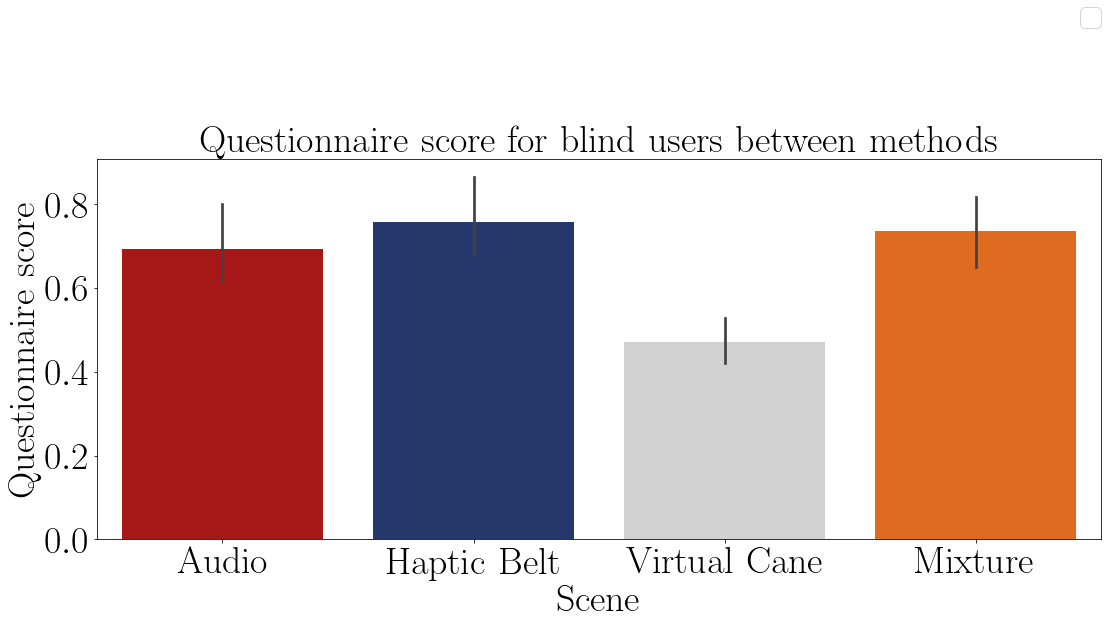
\includegraphics[width = 0.8\linewidth]{Resultados/Questionario/Figuras/png/barplot_questionnaire_scene_blind.png}
    \caption{Barplot of the average questionaire score of the blind participants on each method.}
    \label{fig:barplot_questionnaire_scene_blind}
\end{figure}

Figure \ref{fig:boxplot_quest_blind_scene} brings the questionnaire boxplot, which clearly shows the difference between two groups: haptic belt and virtual cane, and audio and mixture. 

\begin{figure}[!htb]
    \centering
    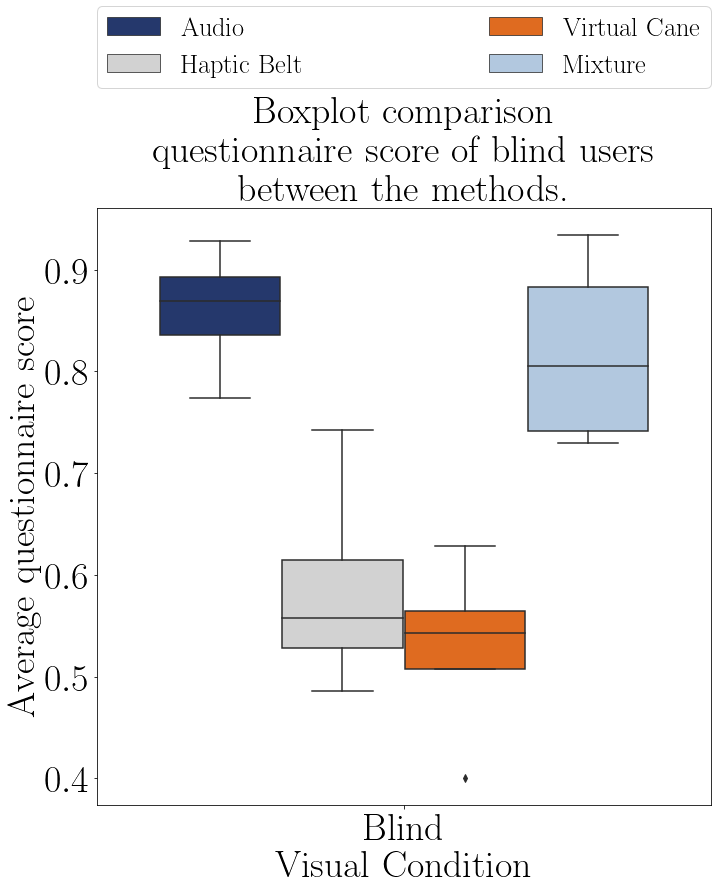
\includegraphics[width = 0.6\linewidth]{Resultados/Questionario/Figuras/png/boxplot_questionnaire_scene_blind.png}
    \caption{Boxplot of the questionaire score of the blind participants grouped by method.}
    \label{fig:boxplot_quest_blind_scene}
\end{figure}

%The Table \ref{tab:questionnaire_average_group_blind} show the the average questionnaire score on each method. It also shows a disatisfaction with the haptic devices alone.
%
%
\begin{table}[!htb]
\centering
\caption{Guidance method questionnaire average score for the blind participants.}
\label{tab:questionnaire_average_group_blind}
\begin{tabular}{lrrrrr}
\toprule
{} & Audio & Haptic Belt & Virtual Cane & Mixture \\
Visual Condition &       &             &              &         \\
\midrule
Blind            &  0.86 &        0.59 &         0.53 &    0.82 \\
\bottomrule
\end{tabular}
\end{table}



Following, Figures \ref{fig:qqplot_questionnaires} and \ref{fig:residplot_questionnaires} shows that the data follows a normal distribution. However, the residual variance is not exactly homogenous among the participants. 

\begin{figure}[!htb]
    \centering
    \begin{minipage}{0.45\textwidth}
        \centering
        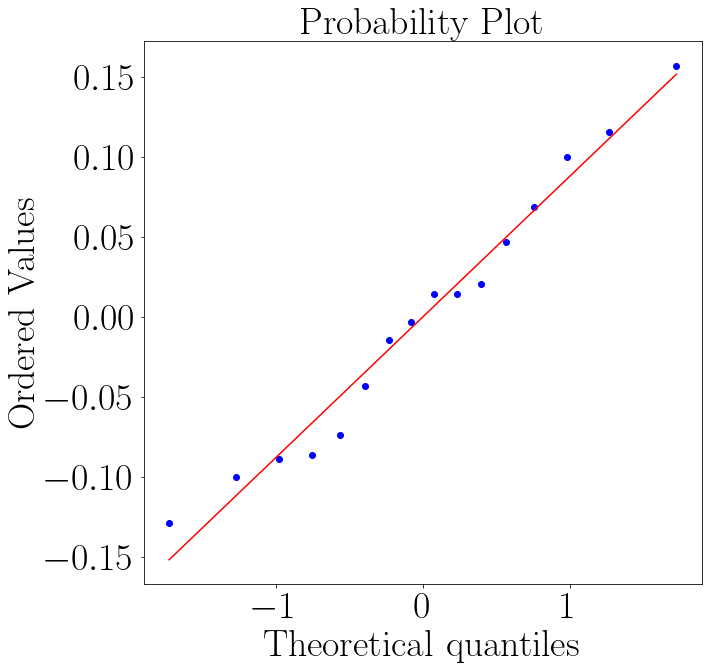
\includegraphics[width = 0.8\linewidth]{Resultados/Questionario/Figuras/png/qqplot_questionnaires.png}
        \caption{QQ plot of the questionnaire score of the blind participants on each method.}
        \label{fig:qqplot_questionnaires}
    \end{minipage}
    \begin{minipage}{0.45\textwidth}
        \centering
        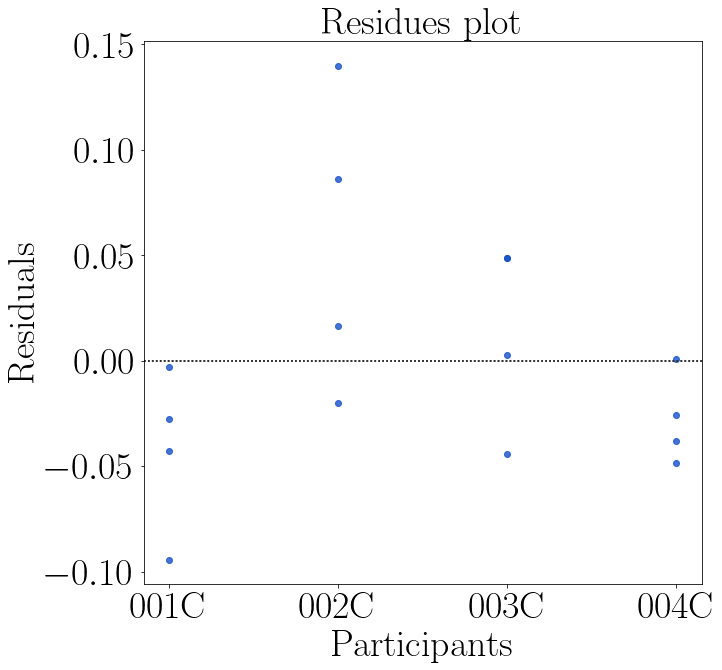
\includegraphics[width = 0.8\linewidth]{Resultados/Questionario/Figuras/png/residplot_questionnaires.png}
        \caption{Residual plot of the questionnaire score the blind participants on each method.}
        \label{fig:residplot_questionnaires}
    \end{minipage}
\end{figure}

The results of ANOVA are presented in Table  \ref{tab:blocanova_questionnaire} and shows that the method, with a p-value of 0.001, is indeed a significant variable that affects the user satisfaction.


\begin{table}[!htb]
\centering
\caption{Anova p-value for the questionnaire score on each method for blinded users.}
\label{tab:blocanova_questionnaire}
\begin{tabular}{lrrrrr}
\toprule
               Source &  Squared sum &  DOF & Squared average &      F & \begin{tabular}[c]{@{}l@{}}P-Value \\ $(F_{0} > F)$\end{tabular} \\
\midrule
Participants (blocks) &        0.042 &    3 &           0.110 &  2.014 &                                                                  \\
               Method &        0.329 &    3 &           0.014 & 15.677 &                                                          0.001** \\
   Experimental error &        0.063 &    9 &           0.007 &        &                                                                  \\
                Total &        0.434 &   15 &                 &        &                                                                  \\
\bottomrule
\end{tabular}
\end{table}



In order to complement the ANOVA analysis, the pairwise comparison of the methods, obtained from the Fisher LSD test, is presented in Table \ref{tab:lsd_questionnaire}. The results show that ‘audio’ and ‘mixture’ are equivalent from the perspective of user satisfaction. All the other comparisons indicate there is a difference between the methods.


\begin{table}[!htb]
\centering
\caption{Cross validation p-value for the questionnaire score on each method for blinded users.}
\label{tab:lsd_questionnaire}
\begin{tabular}{rclr}
\toprule
      \multicolumn{3}{c}{Method} &                                           Analysis \\
\midrule
       Audio & $X$ & Haptic Belt &        $H_1 : \mu_{Audio} \ne \mu_{Haptic Belt}**$ \\
      Audio & $X$ & Virtual Cane &       $H_1 : \mu_{Audio} \ne \mu_{Virtual Cane}**$ \\
           Audio & $X$ & Mixture &                $H_0 : \mu_{Audio} = \mu_{Mixture}$ \\
Haptic Belt & $X$ & Virtual Cane & $H_1 : \mu_{Haptic Belt} \ne \mu_{Virtual Cane}**$ \\
     Haptic Belt & $X$ & Mixture &          $H_0 : \mu_{Haptic Belt} = \mu_{Mixture}$ \\
    Virtual Cane & $X$ & Mixture &     $H_1 : \mu_{Virtual Cane} \ne \mu_{Mixture}**$ \\
\bottomrule
\end{tabular}
\end{table}



Additional to the scores, the participants also expressed their dissatisfaction in the answers to the open questions of the questionnaire, where they commented that the haptic belt and the virtual cane are confusing, are not enough precise, and are very different from what they are used to.

\FloatBarrier
